% !TeX encoding = UTF-8
% !TeX program = xelatex
% !TeX spellcheck = en_US

\documentclass[degree=master, fontset = ubuntu]{thuthesis}
\usepackage{graphicx}
\usepackage{pdfpages}
\usepackage{longtable}
\usepackage{multirow}
  % 学位 degree:
  %   doctor | master | bachelor | postdoc
  % 学位类型 degree-type:
  %   academic(默认)| professional
  % 语言 language
  %   chinese(默认)| english
  % 字体库 fontset
  %   windows | mac | fandol | ubuntu
  % 建议终版使用 Windows 平台的字体编译


% 论文基本配置,加载宏包等全局配置
% !TeX root = ./thuthesis-example.tex

% 论文基本信息配置

\thusetup{
  %******************************
  % 注意:
  %   1. 配置里面不要出现空行
  %   2. 不需要的配置信息可以删除
  %   3. 建议先阅读文档中所有关于选项的说明
  %******************************
  %
  % 输出格式
  %   选择打印版(print)或用于提交的电子版(electronic),前者会插入空白页以便直接双面打印
  %
  output = print,
  %
  % 标题
  %   可使用“\\”命令手动控制换行
  %
  title*  = {Isothermal amplification and frugal open-source hardware as low resource diagnosis gap filler},
  title = {等温扩增以及节俭开源硬件作为低资源诊断的替代品},
  %
  % 学位
  %   1. 学术型
  %      - 中文
  %        需注明所属的学科门类,例如:
  %        哲学、经济学、法学、教育学、文学、历史学、理学、工学、农学、医学、
  %        军事学、管理学、艺术学
  %      - 英文
  %        博士:Doctor of Philosophy
  %        硕士:
  %          哲学、文学、历史学、法学、教育学、艺术学门类,公共管理学科
  %          填写“Master of Arts“,其它填写“Master of Science”
  %   2. 专业型
  %      直接填写专业学位的名称,例如:
  %      教育博士、工程硕士等
  %      Doctor of Education, Master of Engineering
  %   3. 本科生不需要填写
  %
  degree-name  = {工学硕士},
  degree-name* = {Master of Science},
  %
  % 培养单位
  %   填写所属院系的全名
  %
  department = {清华大学深圳国际研究生院},
  %
  % 学科
  %   1. 学术型学位
  %      获得一级学科授权的学科填写一级学科名称,其他填写二级学科名称
  %   2. 工程硕士
  %      工程领域名称
  %   3. 其他专业型学位
  %      不填写此项
  %   4. 本科生填写专业名称,第二学位论文需标注“(第二学位)”
  %
  discipline  = {精准医学与公共健康},
  discipline* = {Precision medicine and healthcare},
  %
  % 姓名
  %
  author  = {弗 朗},
  author* = {Francisco Javier Quero},
  %
  % 指导教师
  %   中文姓名和职称之间以英文逗号“,”分开,下同
  %
  supervisor  = {弥胜利, 教授},
  supervisor* = {Professor Shengli Mi},
  %
  % 副指导教师
  %
  %associate-supervisor  = {陈文光, 教授},
  %associate-supervisor* = {Professor Chen Wenguang},
  %
  % 联合指导教师
  %
  co-supervisor  = {Professor Ariel Lindner},
  co-supervisor* = {Professor Ariel Lindner},
  %
  % 日期
  %   使用 ISO 格式;默认为当前时间
  %
  % date = {2019-07-07},
  %
  % 是否在中文封面后的空白页生成书脊(默认 false)
  %
  include-spine = false,
  %
  % 密级和年限
  %   秘密, 机密, 绝密
  %
  % secret-level = {秘密},
  % secret-year  = {10},
  %
  % 博士后专有部分
  %
  % clc                = {分类号},
  % udc                = {UDC},
  % id                 = {编号},
  % discipline-level-1 = {计算机科学与技术},  % 流动站(一级学科)名称
  % discipline-level-2 = {系统结构},          % 专业(二级学科)名称
  % start-date         = {2011-07-01},        % 研究工作起始时间
}

% 载入所需的宏包

% 定理类环境宏包
\usepackage{amsthm}
% 也可以使用 ntheorem
% \usepackage[amsmath,thmmarks,hyperref]{ntheorem}

\thusetup{
  %
  % 数学字体
  % math-style = GB,  % GB | ISO | TeX
  math-font  = xits  % sitx | xits | libertinus
}

% 可以使用 nomencl 生成符号和缩略语说明
% \usepackage{nomencl}
% \makenomenclature

% 表格加脚注
\usepackage{threeparttable}

% 表格中支持跨行
\usepackage{multirow}

% 固定宽度的表格。
% \usepackage{tabularx}

% 跨页表格
\usepackage{longtable}

% 算法
\usepackage{algorithm}
\usepackage{algorithmic}

% 量和单位
\usepackage{siunitx}

% 参考文献使用 BibTeX + natbib 宏包
% 顺序编码制
\usepackage[sort]{natbib}
\bibliographystyle{thuthesis-numeric}

% 著者-出版年制
% \usepackage{natbib}
% \bibliographystyle{thuthesis-author-year}

% 本科生参考文献的著录格式
% \usepackage[sort]{natbib}
% \bibliographystyle{thuthesis-bachelor}

% 参考文献使用 BibLaTeX 宏包
% \usepackage[style=thuthesis-numeric]{biblatex}
% \usepackage[style=thuthesis-author-year]{biblatex}
% \usepackage[style=apa]{biblatex}
% \usepackage[style=mla-new]{biblatex}
% 声明 BibLaTeX 的数据库
% \addbibresource{ref/refs.bib}

% 定义所有的图片文件在 figures 子目录下
\graphicspath{{figures/}}

% 数学命令
\makeatletter
\newcommand\dif{%  % 微分符号
  \mathop{}\!%
  \ifthu@math@style@TeX
    d%
  \else
    \mathrm{d}%
  \fi
}
\makeatother

% hyperref 宏包在最后调用
\usepackage{hyperref}



\begin{document}

% 封面
\maketitle

% 学位论文指导小组、公开评阅人和答辩委员会名单
% 本科生不需要
% !TeX root = ../thuthesis-example.tex

\begin{committee}[name={学位论文指导小组、公开评阅人和答辩委员会名单}]

  \newcolumntype{C}[1]{@{}>{\centering\arraybackslash}p{#1}}

  \section*{指导小组名单}

  \begin{center}
    \begin{tabular}{C{3cm}C{3cm}C{9cm}@{}}
      李XX & 教授     & 清华大学 \\
      王XX & 副教授   & 清华大学 \\
      张XX & 助理教授 & 清华大学 \\
    \end{tabular}
  \end{center}


  \section*{公开评阅人名单}

  \begin{center}
    \begin{tabular}{C{3cm}C{3cm}C{9cm}@{}}
      刘XX & 教授   & 清华大学                    \\
      陈XX & 副教授 & XXXX大学                    \\
      杨XX & 研究员 & 中国XXXX科学院XXXXXXX研究所 \\
    \end{tabular}
  \end{center}


  \section*{答辩委员会名单}

  \begin{center}
    \begin{tabular}{C{2.75cm}C{2.98cm}C{4.63cm}C{4.63cm}@{}}
      主席 & 赵XX                  & 教授                    & 清华大学       \\
      委员 & 刘XX                  & 教授                    & 清华大学       \\
          & \multirow{2}{*}{杨XX} & \multirow{2}{*}{研究员} & 中国XXXX科学院 \\
          &                       &                         & XXXXXXX研究所  \\
          & 黄XX                  & 教授                    & XXXX大学       \\
          & 周XX                  & 副教授                  & XXXX大学       \\
      秘书 & 吴XX                  & 助理研究员              & 清华大学       \\
    \end{tabular}
  \end{center}

\end{committee}



% 也可以导入 Word 版转的 PDF 文件
% \begin{committee}[file=figures/committee.pdf]
% \end{committee}


% 使用授权的说明 DESCOMENTAR
%\copyrightpage
% 将签字扫描后授权文件 scan-copyright.pdf 替换原始页面
% \copyrightpage[file=scan-copyright.pdf]

\frontmatter
% !TeX root = ../thuthesis-example.tex

% 中英文摘要和关键字

\begin{abstract}
  精明的决策在妥善处理大流行病方面具有重要作用。为此,对人群进行全面和及时的诊断是必不可少的。不幸的是,2019年冠状病毒大流行(COVID-19)证明了在资源匮乏的地区缺乏有效、简便和便宜的诊断解决方案。
  
  本论文将介绍一种快速、敏感、价格实惠和冷链独立解决方案,该解决方案可在Low to Middle-Income Countries (LMICs)的临床样本中有效地检测出SARS-CoV-2。我们的技术被命名为CoronaDetective,可以以不到2美元的价格扩增SARS-CoV-2病毒基因组。CoronaDetective使用等温扩增技术,特别是Quenching of Unincorporated Amplification Signal Reporters in Reverse-Transcription Loop-Mediated Isothermal Amplification (QUASR-LAMP),来扩增病毒RNA并发出荧光信号。此外,CoronaDetective已被证明对加纳和智利的许多临床样本有效。
  
  其次,我们设计并生产了两个开源硬件,一种是带有集成透射器水浴,另一种是实时LAMP机,主要目的是对放大效果进行定性和定量分析。这两个设备的设计均是开源的,很容易使用广泛的数字制造技术进行复制,便于在世界任何地方生产。事实证明,5美元的水浴与标准的实验室设备在孵化和分析反应方面的效果相同。尽管还有待进一步研究,但实时LAMP机显示了这种硬件的潜力,可以用50美元的成本进行定量分析。  
  
  我们希望,有了这些技术,在减少我们星球的诊断差距方面贡献自己的一份力。

  % 关键词用“英文逗号”分隔,输出时会自动处理为正确的分隔符
  \thusetup{
    keywords = {等温扩增 1, 开源硬件 2, 冠状病毒 3, 低资源诊断法 4, 节俭的科学 5},
  }
\end{abstract}
  .
\begin{abstract*}
Informed decision-making has a vital role in the proper management of pandemics. For this, a comprehensive and timely diagnosis of the population is essential. Unfortunately, the recent 2019 coronavirus pandemic (COVID-19) evidenced a lack of robust, simple and inexpensive diagnostic solutions that can be implemented in areas where resource scarcity becomes the bottleneck.
  
 This thesis will describe a fast, sensitive, affordable and cold-chain independent solution that allows robust detection of SARS-CoV-2 in clinical samples at Low to Middle-Income Countries (LMICs). Our technology starts with the CoronaDetective reactions, that allows the amplification of the SARS-CoV-2 viral genome by less than \$2. CoronaDetective uses isothermal amplification technologies, particularly Quenching of Unincorporated Amplification Signal Reporters in Reverse-Transcription Loop-Mediated Isothermal Amplification (QUASR-LAMP),  to amplify the viral RNA and generate a fluorescent signal. Furthermore, CoronaDetective has been proven to work with many clinical samples in Ghana and Chile.
  
Secondly, two open-source hardware devices, a water bath with an integrated transilluminator and a Real-Time LAMP machine, have been designed and produced with the primary goal of performing the qualitative and quantitative analysis of the amplification. The designs of both devices are open source and easy to replicate using widespread digital fabrication techniques, facilitating their production in any part of the world. The \$5 water bath has been proven to work equally to standard laboratory equipment for incubating and analyzing the reactions. Although more work is still needed, the Real-Time LAMP machine shows the potential of this hardware to perform the quantitative analysis at the cost of \$50. 
  
 We hope that, with these technologies, we add our little grain of sand in reducing the diagnosis gap in our planet.


  % Use comma as separator when inputting
  \thusetup{
    keywords* = {Isothermal amplification, Open-Source Hardware, Coronavirus, Low-Resources Diagnostics, Frugal science},
  }
\end{abstract*}


% 目录
\tableofcontents

% 插图和附表清单
% 本科生的插图索引和表格索引需要移至正文之后、参考文献前
\listoffiguresandtables  % 插图和附表清单(仅限研究生)
%\listoffigures           % 插图清单
%\listoftables            % 附表清单

% 符号对照表
% !TeX root = ../thuthesis-example.tex

\begin{denotation}[3cm]
  \item[PI] 聚酰亚胺
  \item[MPI] 聚酰亚胺模型化合物,N-苯基邻苯酰亚胺
  \item[PBI] 聚苯并咪唑
  \item[MPBI] 聚苯并咪唑模型化合物,N-苯基苯并咪唑
  \item[PY] 聚吡咙
  \item[PMDA-BDA] 均苯四酸二酐与联苯四胺合成的聚吡咙薄膜
  \item[MPY] 聚吡咙模型化合物
  \item[As-PPT] 聚苯基不对称三嗪
  \item[MAsPPT] 聚苯基不对称三嗪单模型化合物,3,5,6-三苯基-1,2,4-三嗪
  \item[DMAsPPT] 聚苯基不对称三嗪双模型化合物(水解实验模型化合物)
  \item[S-PPT] 聚苯基对称三嗪
  \item[MSPPT] 聚苯基对称三嗪模型化合物,2,4,6-三苯基-1,3,5-三嗪
  \item[PPQ] 聚苯基喹噁啉
  \item[MPPQ] 聚苯基喹噁啉模型化合物,3,4-二苯基苯并二嗪
  \item[HMPI] 聚酰亚胺模型化合物的质子化产物
  \item[HMPY] 聚吡咙模型化合物的质子化产物
  \item[HMPBI] 聚苯并咪唑模型化合物的质子化产物
  \item[HMAsPPT] 聚苯基不对称三嗪模型化合物的质子化产物
  \item[HMSPPT] 聚苯基对称三嗪模型化合物的质子化产物
  \item[HMPPQ] 聚苯基喹噁啉模型化合物的质子化产物
  \item[PDT] 热分解温度
  \item[HPLC] 高效液相色谱(High Performance Liquid Chromatography)
  \item[HPCE] 高效毛细管电泳色谱(High Performance Capillary lectrophoresis)
  \item[LC-MS] 液相色谱-质谱联用(Liquid chromatography-Mass Spectrum)
  \item[TIC] 总离子浓度(Total Ion Content)
  \item[\textit{ab initio}] 基于第一原理的量子化学计算方法,常称从头算法
  \item[DFT] 密度泛函理论(Density Functional Theory)
  \item[$E_a$] 化学反应的活化能(Activation Energy)
  \item[ZPE] 零点振动能(Zero Vibration Energy)
  \item[PES] 势能面(Potential Energy Surface)
  \item[TS] 过渡态(Transition State)
  \item[TST] 过渡态理论(Transition State Theory)
  \item[$\increment G^\neq$] 活化自由能(Activation Free Energy)
  \item[$\kappa$] 传输系数(Transmission Coefficient)
  \item[IRC] 内禀反应坐标(Intrinsic Reaction Coordinates)
  \item[$\nu_i$] 虚频(Imaginary Frequency)
  \item[ONIOM] 分层算法(Our own N-layered Integrated molecular Orbital and molecular Mechanics)
  \item[SCF] 自洽场(Self-Consistent Field)
  \item[SCRF] 自洽反应场(Self-Consistent Reaction Field)
\end{denotation}



% 也可以使用 nomencl 宏包,需要在导言区
% \usepackage{nomencl}
% \makenomenclature

% 在这里输出符号说明
% \printnomenclature[3cm]

% 在正文中的任意为都可以标题
% \nomenclature{PI}{聚酰亚胺}
% \nomenclature{MPI}{聚酰亚胺模型化合物,N-苯基邻苯酰亚胺}
% \nomenclature{PBI}{聚苯并咪唑}
% \nomenclature{MPBI}{聚苯并咪唑模型化合物,N-苯基苯并咪唑}
% \nomenclature{PY}{聚吡咙}
% \nomenclature{PMDA-BDA}{均苯四酸二酐与联苯四胺合成的聚吡咙薄膜}
% \nomenclature{MPY}{聚吡咙模型化合物}
% \nomenclature{As-PPT}{聚苯基不对称三嗪}
% \nomenclature{MAsPPT}{聚苯基不对称三嗪单模型化合物,3,5,6-三苯基-1,2,4-三嗪}
% \nomenclature{DMAsPPT}{聚苯基不对称三嗪双模型化合物(水解实验模型化合物)}
% \nomenclature{S-PPT}{聚苯基对称三嗪}
% \nomenclature{MSPPT}{聚苯基对称三嗪模型化合物,2,4,6-三苯基-1,3,5-三嗪}
% \nomenclature{PPQ}{聚苯基喹噁啉}
% \nomenclature{MPPQ}{聚苯基喹噁啉模型化合物,3,4-二苯基苯并二嗪}
% \nomenclature{HMPI}{聚酰亚胺模型化合物的质子化产物}
% \nomenclature{HMPY}{聚吡咙模型化合物的质子化产物}
% \nomenclature{HMPBI}{聚苯并咪唑模型化合物的质子化产物}
% \nomenclature{HMAsPPT}{聚苯基不对称三嗪模型化合物的质子化产物}
% \nomenclature{HMSPPT}{聚苯基对称三嗪模型化合物的质子化产物}
% \nomenclature{HMPPQ}{聚苯基喹噁啉模型化合物的质子化产物}
% \nomenclature{PDT}{热分解温度}
% \nomenclature{HPLC}{高效液相色谱(High Performance Liquid Chromatography)}
% \nomenclature{HPCE}{高效毛细管电泳色谱(High Performance Capillary lectrophoresis)}
% \nomenclature{LC-MS}{液相色谱-质谱联用(Liquid chromatography-Mass Spectrum)}
% \nomenclature{TIC}{总离子浓度(Total Ion Content)}
% \nomenclature{\textit{ab initio}}{基于第一原理的量子化学计算方法,常称从头算法}
% \nomenclature{DFT}{密度泛函理论(Density Functional Theory)}
% \nomenclature{$E_a$}{化学反应的活化能(Activation Energy)}
% \nomenclature{ZPE}{零点振动能(Zero Vibration Energy)}
% \nomenclature{PES}{势能面(Potential Energy Surface)}
% \nomenclature{TS}{过渡态(Transition State)}
% \nomenclature{TST}{过渡态理论(Transition State Theory)}
% \nomenclature{$\increment G^\neq$}{活化自由能(Activation Free Energy)}
% \nomenclature{$\kappa$}{传输系数(Transmission Coefficient)}
% \nomenclature{IRC}{内禀反应坐标(Intrinsic Reaction Coordinates)}
% \nomenclature{$\nu_i$}{虚频(Imaginary Frequency)}
% \nomenclature{ONIOM}{分层算法(Our own N-layered Integrated molecular Orbital and molecular Mechanics)}
% \nomenclature{SCF}{自洽场(Self-Consistent Field)}
% \nomenclature{SCRF}{自洽反应场(Self-Consistent Reaction Field)}



% 正文部分
\mainmatter
% !TeX root = ../thuthesis-example.tex

\chapter{Introduction}

In 1985 Kary Mullis revolutionised the nucleic acid research field with the Nobel awarded Polymerase Chain Reaction (PCR) technique \cite{saiki_enzymatic_1985}. Since that moment humankind was able to replicate \emph{in vitro} the first step of the biology central dogma, making it possible to amplify, detect and even edit DeoxyriboNucleic Acid (DNA). Later, PCR has been the precursor of a long family of nucleic acid amplification procedures that have taken one step further the capabilities of the technique.

Diagnostics and biosensing are some of the most affected fields by the PCR invention. As a Nucleic Acid Amplification Test (NAAT), and in contrast with other non-nucleic-acid based techniques, PCR has the key advantage of replicating one of the molecules present in the target, and therefore, generating a highly specific exponential signal. In the end, this allows NAATs to reach robust levels of sensibility and specificity. 

Even though PCR-based NAATs have become the gold standard in the biosensing field\cite{oliveira_isothermal_2021}, they have a main limiting factor; they require a highly expensive environment to perform accurately, including a fully equipped molecular lab and well-trained personnel. 
\linebreak
\linebreak

\begin{figure}[b]
    \centering
    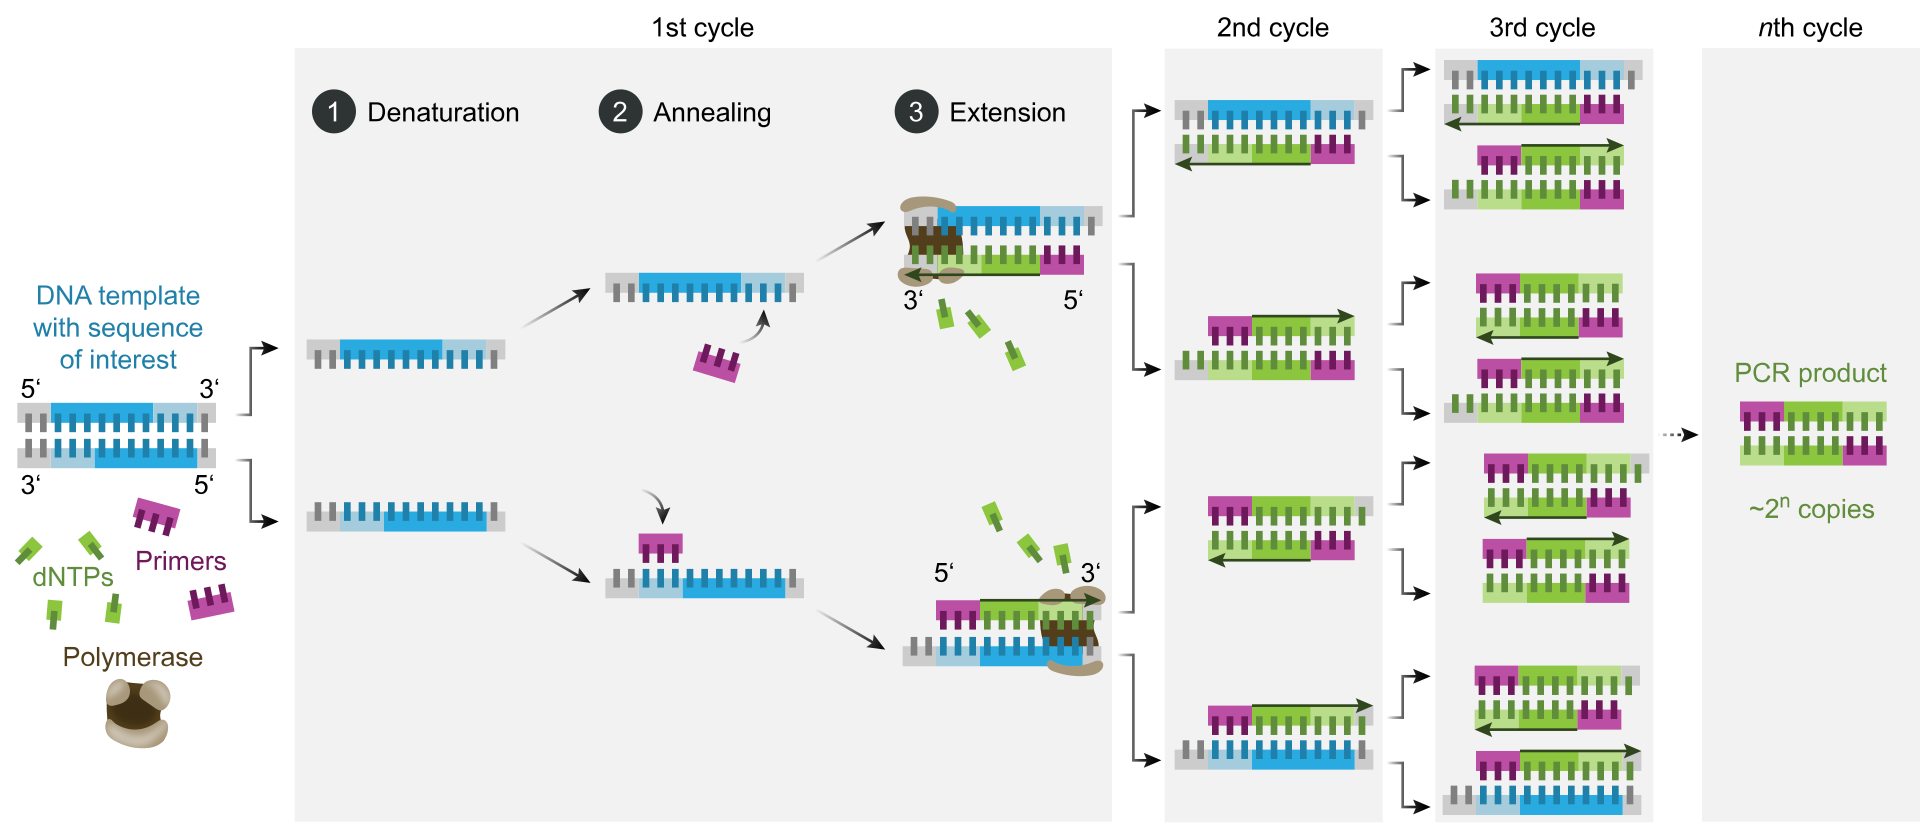
\includegraphics[width=1\textwidth]{figures/PCR.png}
    \caption[Scheme of PCR amplification working principle.] {Scheme of PCR amplification working principle. Adapted from Enzoklop, CC BY-SA 4.0 , via Wikimedia Commons.}
    \label{fig:PCR}
\end{figure}


\section{The problem of thermal cycling}

Through the PCR, the reactions are submitted to cycles of heat and cold, which helps couple and uncouple the double strand of nucleic acids and create the conditions that the reagents need to interact with the DNA. 

When it comes to diagnosis the gold standard is Real-Time PCR (RT-PCR)\cite{world_health_organization_laboratory_2016}\cite{world_health_organization_interim_2015}\cite{world_health_organization_recommendations_2021}. The RT-PCR is an evolution of PCR, where the amplification of DNA is designed to give a fluorescent signal that is measured cyclically during the reaction. The amount of signal at a certain time is proportional to the initial quantity of target in the sample, and therefore, the amount of target can be quantified by comparing the signal with the fluorescence of a control.For carrying out the amplification, a \emph{thermocycler} is required, which provide fast temperature switching making the system efficient and drastically reducing the required time. In the case of RT-PCR, the machine used is called \emph{Real-Time thermocycler}, which additionally measures the signal fluorescence cyclically. Standard Real-time thermocyclers cost around 40.000\$, are not portable and their use requires specialized molecular biology training.

All of these ends up generating so many difficulties to implement these technologies for diagnoses in Low to Middle-Income Countries (LMIC), where, paradoxically, they are more needed.

\section{The isothermal Nucleic Acid Amplification Tests}

In a nutshell, the isothermal Nucleic Acid Amplification Test (iNAAT) are  NAATs that happen at a constant temperature. This key factor generates a huge improvement in the applicability of the PCR-based NAATs because there is no longer a need for a thermocycler and the reactions can be carried out just in a simple water bath or incubator. 

Even if initially it might appear challenging, nature always works amplifying nucleic acids at a constant temperature. Indeed, this technology replicates solutions that are already present in nature to solve the strand unfolding challenge. Contrary to current thinking, the isothermal amplifications preceded the invention of PCR. In 1965 Spiegelman laboratory used purified RNA-dependent-RNA-polymerase from the bacteriophage Qbeta (Qb) to exponentially amplify the phage genome \emph{in vitro} \cite{spiegelman_synthesis_1965}. The group later discovered that this method generates the accumulation of numerous errors, which led this technique to be used as the first attempt for extracellular evolution. However, when it comes to efficient DNA amplification, the technique was later on completely eclipsed by PCR.

\begin{figure}[b]
    \centering
    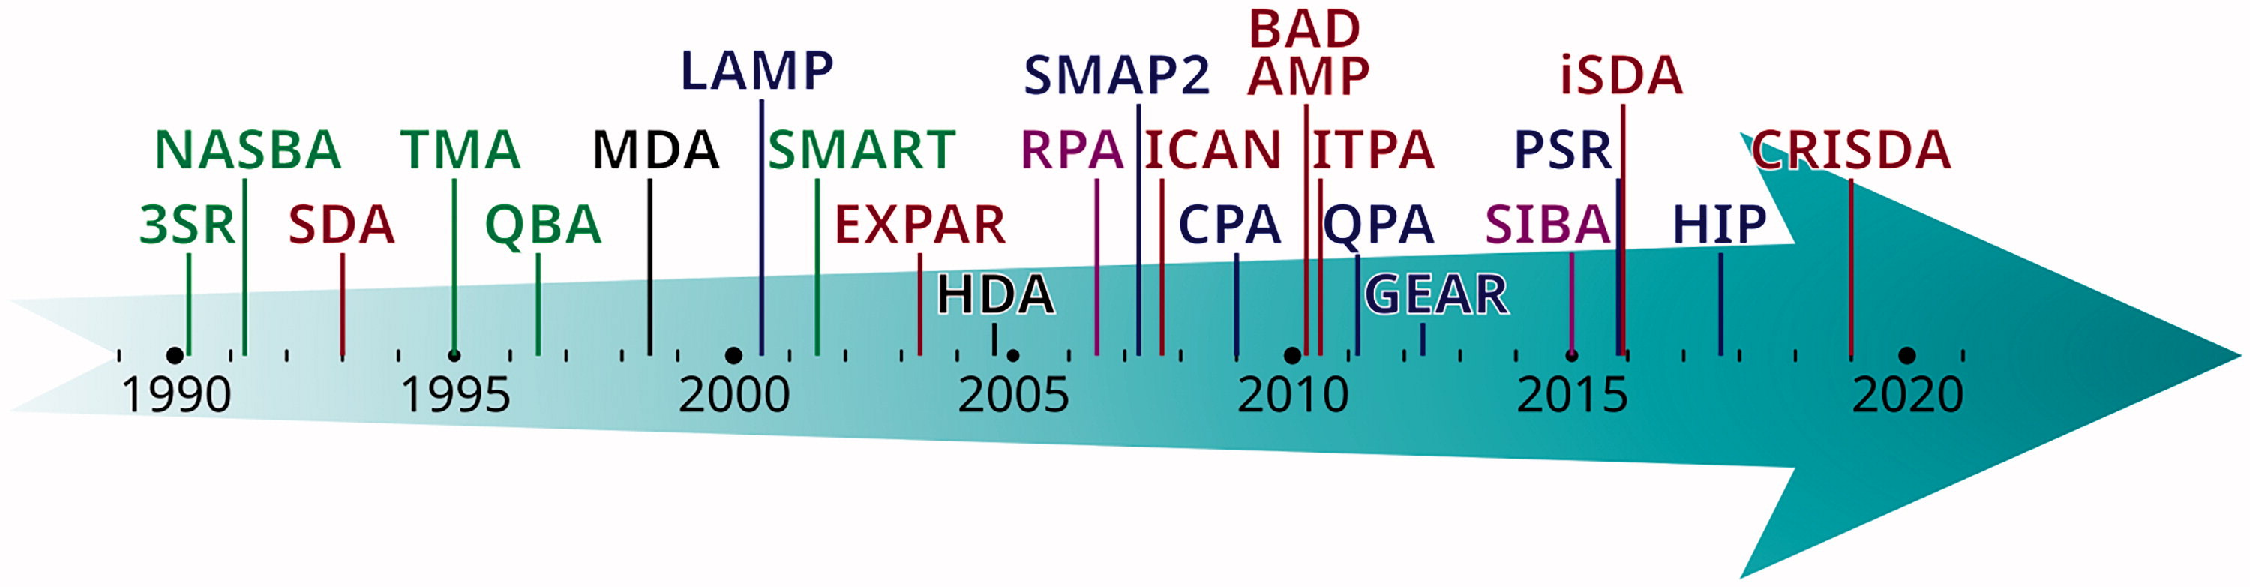
\includegraphics[width=1\textwidth]{data/iso_amp_methods.pdf}
    \caption[Timeline of isothermal nucleic acid amplification methods.]{Timeline of isothermal nucleic acid amplification methods. The colour of the amplification method indicates the underlying mechanism; promoter-based in green, nicking-based in red, refolding-based in blue, strand-invasion-based in purple and unique mechanisms in black. Image taken from Glökler et al. 2021\cite{glokler_isothermal_2021}.}
    \label{fig:iso_amp_methods}
\end{figure}

The first modern (post-PCR era) isothermal amplification method that gained attention was the self-sustained sequence replication (3SR) published in 1990 \cite{guatelli_isothermal_1990} shortly followed by the very similar nucleic acid sequence-based amplification (NASBA) in 
1991 \cite{compton_nucleic_1991} and the transcription-mediated amplification (TMA) in 1995 \cite{kacian_nucleic_1995}. They paved the way for the more than 20 isothermal amplification methods existing nowadays. The most important ones, and their working principle, are illustrated in Figure 1.2 \cite{glokler_isothermal_2021}.


%Broad explanation of isothermal amplifications
Isothermal amplifications can be categorized in numerous ways. One possibility is to separate the iNAATs that generates new strands exponentially from the ones that produce them in a linear way. Because the iNAATs that works in an exponential way are much more powerful in terms of a quick diagnosis, they dominated the diagnosis field over the linear ones.

Another way of classifying them, more useful for understanding the bigger picture of iNAATs, separates the different techniques by their underlying working principle\cite{glokler_isothermal_2021}. \linebreak

Broadly there are four different categories, illustrated in Figure 1.3:

\begin{enumerate}
   \item \emph{Promoter-based mechanisms} include target sequences for RNA polymerases in the original sequence that led to the amplification by transcription. The most well known and documented iNAAT in this category is NASBA\cite{compton_nucleic_1991}. 
   \item \emph{Nicking-based mechanisms} employs nicking enzymes to  break one of the strands to start the replication process. The resulting 3' end, left open by the enzyme, can be later used by a polymerase to start the amplification. The original method was called Strand Displacement Amplification (SDA)\cite{ness_isothermal_2003} and inspired by it, many variants have been developed.
   \linebreak
   \linebreak
   \item \emph{Refolding-based mechanisms} employs self-priming of the amplified sequences by designing the initial primers to target two different sequences in the sample, and therefore folding back generating hairpins and initiating two different amplifications. The generation of the LAMP method by the Notomi laboratory kick-started a whole plethora of similar methods in this category\cite{notomi_loop-mediated_2000}. 
   \item \emph{Strand invasion-based mechanisms} is the most novel way to perform exponential isothermal amplification. It is based on the working principle of natural recombinases, that binds to single-stranded nucleic acids, and targets double-stranded complementary sequences by a strand invasion mechanism. The most mature technology in this category is Recombinase Primed Amplification (RPA)\cite{piepenburg_dna_2006}.
\end{enumerate}

%Image that explains the different methods
\begin{figure}[b]
    \centering
    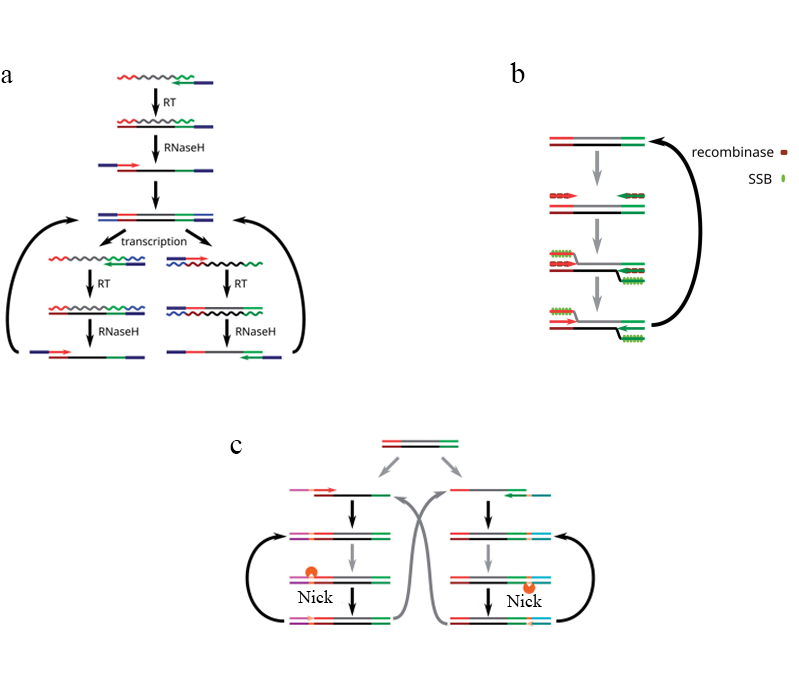
\includegraphics[width=1\textwidth]{data/iNAATs.png}
    \caption[Representation of isothermal amplification techniques]{A scheme that represents the working principles of isothermal amplification techniques based in a) promoter amplification, b) strand invasion and c) nicking enzymes. Refolding based mechanism is separated and illustrated in Figure 1.4. Image adapted from Glökler et al. 2021\cite{glokler_isothermal_2021}.}
    \label{fig:commercial iNAATs}
\end{figure}

Despite all this panorama of iNAATs developed to date, just a few of them have been significantly applied to real scenarios. In Figure 1.4 can be observed the comparison between the different tests in terms of their development state. The table A.2.1 of the appendix A gathers the main commercial kits based on iNAATs.

NASBA was one of the first techniques to not only be developed but also applied in real diagnosis scenarios. Because of its working principle, in its origins, NASBA was handy to detect viruses\cite{rutjes_real-time_2006}. A notorious recent application was its adaption to monitor the recycled water in the International Space Station\cite{bechy-loizeau_assessment_2015}. NASBA has been proven to be more sensitive and less prone to inhibitory substances than PCR\cite{rutjes_real-time_2006}, and immune to contamination by DNA, because the temperature is kept below the DNA melting point, so strand displacement does not occur\cite{simpkins_rna_2000}. Still, the high cost of the reaction (~26\$ per test\cite{oliveira_isothermal_2021}) and the need to optimize 3 different enzymes have prevented the development of commercial products based on NASBA.

\begin{figure}[b]
    \centering
    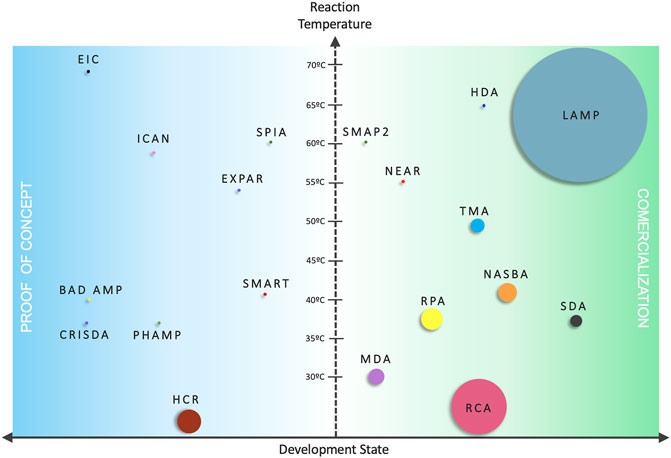
\includegraphics[width=0.85\textwidth]{figures/commercial kits.jpg}
    \caption[Comparison between iNAATs working principles and their development state.]{Comparison between iNAATs working principles and their development state. The vertical axis represents the reaction temperature and the horizontal axis how developed is the technology, from methods not developed far away from academic concepts (Blue), to already commercialized systems (Green). The size of the circles represents the number of scientific items in literature. Image obtained from Oliveira et al. 2021\cite{oliveira_isothermal_2021}.}
    \label{fig:development state}
\end{figure}

%RCA
Rolling Circle Amplification (RCA) is also one of the earlier developed iNAATs \cite{fire_rolling_1995} and even though it has some great advantages, such as the low temperature (23-60ºC) or its ability to work in complex biological matrices (allowing for molecular-level detection in living cells\cite{konry_ultrasensitive_2011}) the linear amplification profile has prevented RCA-based products to reach the diagnosis market.

%RPA
Nowadays RPA is one of the iNAATs that have more potential to win the race for the next "Gold Standard" in nucleic acid amplification \cite{oliveira_isothermal_2021}. Some of the key characteristics that justify the bloom of RPA are the low incubation temperature (37-42ºC), a PCR level sensitivity (Limit of Detection (LoD) between 10-20 copies of target DNA) and one of the fastest times-to-complete reactions (10-20 mins)\cite{kunze_-chip_2016}. Moreover, RPA assays can work with low sample volumes, seems to be robust under high concentrations of PCR inhibitors, and don't require an initial DNA denaturalization step\cite{twist_dx_recombinase_2017}\cite{kersting_rapid_2014}\cite{deng_bioanalytical_2015-1}.

These characteristics made RPA be one of the iNAATs that have the larger commercial potential. Indeed, the technology was already patented in 2005 by TwistDx (later acquired by Abbott Diagnostics). The ambit of application was originally the US and soon they expanded to the rest of the world\cite{armes_recombinase_2007}.

Apart from the patented commercialization, RPA has some limiting factors for its applicability. The fact that RPA uses a complex mix of 3 enzymes makes the system less stable and prone to lose efficiency, getting the enzymes degraded over time. Furthermore, the requirement of 3 enzymes, makes the systems complex to optimize and produce. 

Following the lessons learnt from the SARS-CoV-2 pandemic, if global needs are to be met, we cannot rely only on manufacturers primarily in high-income countries (HICs) \cite{medecins_sans_frontieres_local_2021}. 

The fact that not only one but three enzymes need to be produced, characterized and optimized, make RPA far from a short or mid-term global applicability. A simpler system, with the same potential but dependent on fewer enzymes, is required.

\section{Loop-Mediated Isothermal Amplification}

%Breve introduccion a LAMP
Loop-Mediated Isothermal Amplification (LAMP)\cite{notomi_loop-mediated_2000} is the most widely spread iNAAT, referenced in approximately 3700 scientific publications and 17 clinical trials\cite{clinicaltrialsgov_loop-mediated_2022}. Perhaps one of the most relevant acknowledgements along all the LAMP history has been its recognition by the World Health Organization to fulfil all the requirements for an \emph{ideal} diagnostics NAAT\cite{wong_loop-mediated_2018}.

%Principio de amplificación.
%Mejora con seis Primers

The working principle of LAMP can be included in the above categorization as a \emph{strand refolding mechanism} and is exemplified in Figure 1.5. LAMP relies on the strand-displacement activity of a DNA polymerase (Traditionally the Bst polymerase\cite{notomi_loop-mediated_2000}) and a special set of 4 different primers targeting 6 different regions. This is possible due to the special design of the so-called "Inner primers", composed of two sequences that align with different regions in the target strand, one in the forward sequence and the other in the reverse, and an optional separating sequence between them. Within the amplification, the inner primers re-align with their own strand, self-priming and generating a new origin of amplification. The second pair of primers, the forward and reverse outer primers, align in the external regions of the amplicon promoting the displacement of the inner primers amplified product and speeding up the reaction. 

\begin{figure}[b]
    \centering
    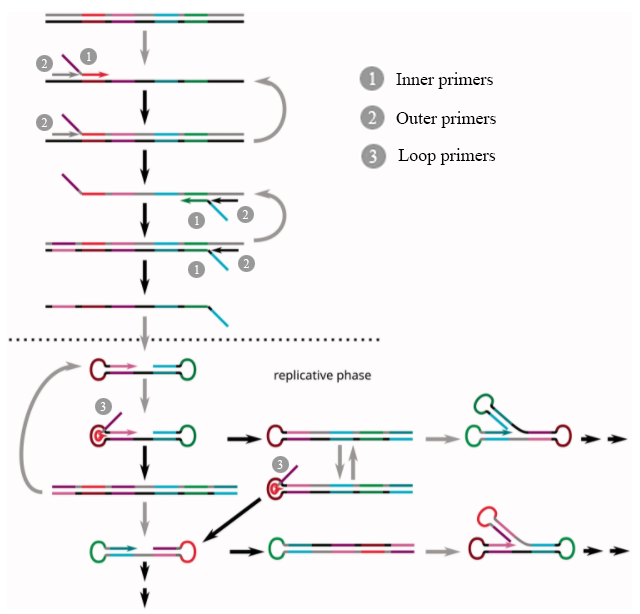
\includegraphics[width=0.8\textwidth]{figures/lamp.png}
    \caption[Explanation of the LAMP working principle.]{Explanation of the LAMP working principle. Image adapted from Glökler et al. 2021 \cite{glokler_isothermal_2021}}.
    \label{fig:LAMP}
\end{figure}

This loop-based elongation generates many different concatemeric sequences with multiple origins of amplification, that in three-dimension acquire a cauliflower shape and possess a high resistance against degradation. In a later improvement of the technique, a third pair of primers were included. These primers target the loop region generated by the Inner primers, highly accelerating the reaction\cite{nagamine_accelerated_2002}.
%Figura de como funciona y leyenda de cada primer

%Caracteristicas
This principle of work endows LAMP with the ability to detect 1 copy per microliter\cite{zhang_lamp---chip_2019}, 10 to 100 fold more sensitive than PCR, with an amplification time of less than 1h around 63-65ºC and yielding $10^9$ copies\cite{notomi_loop-mediated_2000}. Furthermore, LAMP is resistant to inhibitory substances and doesn't require, like many other iNAATs, an initial denaturation step at 95ºC\cite{enomoto_rapid_2005}\cite{kaneko_tolerance_2007}.
%Aplicación
When it comes to the applicability, the original family of LAMP patents recently expired\cite{tsugunori_notomi_hase_tetsu_process_2000}, coinciding with  the beginning of the global SARS-CoV-2 pandemic. Indeed, just within the framework of the pandemic, at least 13 diagnosis kits based in LAMP have addressed the \emph{In Vitro Diagnosys} (IVD) certification at least  in one of the main regulatory agencies in the world \cite{find_sars-cov-2_2022}, and 4 more are in development \cite{find_sars-cov-2_2022-1}. In the global infectious diseases panorama, LAMP kits have been commercialized for Tuberculosis, Malaria and Leishmania among others\cite{oliveira_isothermal_2021}. 

To summarize, there is an exponential growth of the LAMP applications and a market in expansion, partially boosted by the pandemic need for simpler and more affordable diagnosis methods. 

\section{The problem of false positives}

Even though the above-mentioned advantages, traditional LAMP face a main obstacle to being implemented; When it comes to the real application the reactions can easily come out as false positives. This problem has been partially linked with carryover contamination by the highly-stable cauliflower-shaped LAMP amplicons\cite{gao_pullulan_2019} as well as the aberrant  amplification started by secondary structures originated by the complex mix of six primers. 

Another important factor in the generation of false positives is the Bst polymerase structure. As the polymerase works at high magnesium concentrations (4-8mM) the binding between the enzyme and the substrate is allowed to be more flexible, therefore giving the Bst the ability to amplify a broader number of substrates. When it comes to the diagnosis this has pros and cons. On one hand, the Bst polymerase can amplify a broader number of nucleic acids templates (as RNA or non-standard nucleic acids) even in the presence of amplification inhibitors\cite{glokler_isothermal_2021} which allows, for example, a robust viral RNA amplification by the so-called \emph{Reverse Transcription} LAMP. On the other hand, this contributes to the so-called false positives, as the polymerase is described to not only perform non-specific amplifications but even \emph{ab initio} synthesis\cite{zyrina_ab_2014}.

Apart from the above-mentioned origins of contamination, the false positive is amplified by the traditional LAMP signal generation methods. The initially proposed method consists of the direct naked-eye observation of turbidity generation, created by the high yields of LAMP amplified DNA \cite{notomi_loop-mediated_2000}. This is not only a difficult task for the human eye, that introduce a relevant human error in the system, but also a process that will give a positive result independently of the amplified DNA sequence in the tube.

As the DNA amplification results in a PH change, PH indicators (typically phenol red) can be used to get a positive signal once the amplification is performed. This method has been used as a standard in the LAMP industry for the last years and is the one applied in the NEB WarmthStart kit\cite{new_england_biolabs_warmstart_2022}, the most spread MasterMix across laboratories. This method is not only sensible to unspecific off-target amplification but it is also described to be affected by external factors as the sample composition\cite{uribe-alvarez_low_2021}.

Intercalant dyes, commonly used in PCR-based amplification, can inhibit the amplification as they partially bind to the DNA at the incubation temperature. Even if some intercalant dyes have been described to avoid the inhibition (SYTO9/SYTO82)\cite{oscorbin_comparison_2016} the problem of unspecific signal generation is still there.

Apart from the impact in the method specificity, this unspecific amplification  further means that the above detection techniques cannot be multiplexed, eventually allowing the detection of more than one target in a single reaction. 

Other techniques have been developed based on strand displacement of a quencher bound to a probe targeting the loop region of the amplicon (DARQ\cite{tanner_simultaneous_2012} and OSD\cite{bhadra_high-surety_2020}) mimicking the working mechanism of the PCR TaqMan probes technology. The problem of these techniques is the risk of inhibiting the reaction, as the sequences used for generating the signal compete with the ones used for amplification\cite{ball_quenching_2016}.

All the above-mentioned difficulties settled the basis for the need for a specific LAMP amplification method.

\section{Quenching of Unincorporated Amplification Signal Reporters LAMP}

Quenching of Unincorporated Amplification Signal Reporters LAMP (QUASR-LAMP) is a target-specific method for generating a signal out of a LAMP amplification. QUASR-LAMP can be considered as an evolution of the above mentioned DARQ. It uses the same principle but takes advantage of quencher probes designed with lower melting temperature (Tm) that don't inhibit the reaction and keep more signal to noise ratio\cite{ball_quenching_2016}.

In Figure 1.6, the QUASR-LAMP working principle is exemplified. A fluorophore is attached to the 5' end of one of the 6 primers. A probe is designed to be complementary to the fluorescent probe with a melting temperature significantly lower than the reaction one (At least 5 ºC less)\cite{ball_quenching_2016}. In the absence of a specific amplified target, the probe keeps joined to the quencher, and the fluorescence is inhibited. When the target is amplified, its complementarity for the fluorescent probe is considerably more significant than the quenching probe, displacing their alignment and separating the quencher from the fluorophore and generating the signal. Different targets can be multiplexed with different fluorescence colours.

Combining the simplicity and affordability of the iNAATs, together with the specificity and sensitivity of PCR, QUASR-LAMP has all the characteristics required for a robust diagnose test. Alongside a proper hardware, that allows both the incubation and analysis of the reactions, the potential of QUASR-LAMP is huge and spread in fields such as infectious disease diagnosis for human health and agriculture, water purity testing and food safety analysis among others.

\begin{figure}[h]
    \centering
    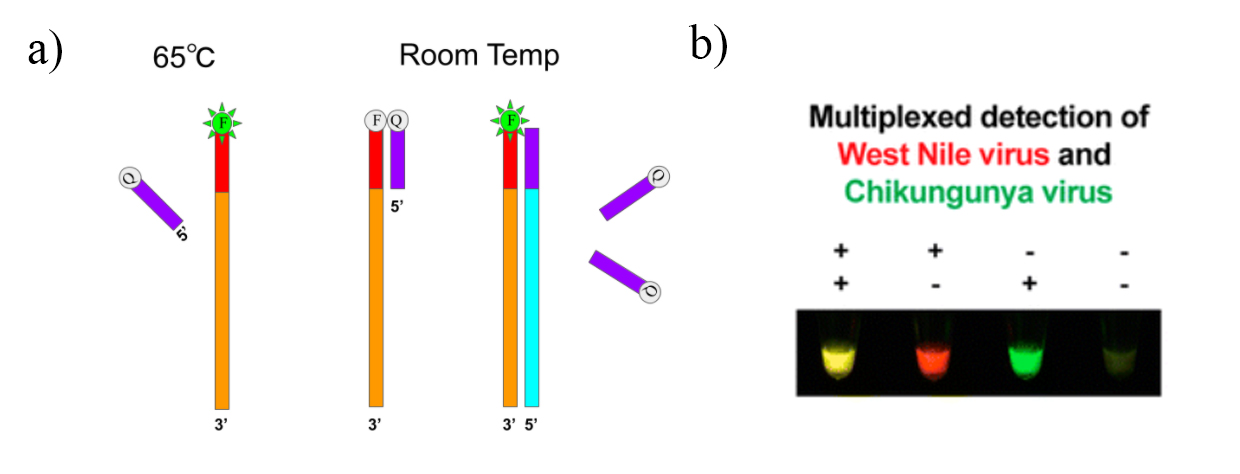
\includegraphics[width=1\textwidth]{figures/QUASR.JPG}
    \caption[Graphical summary of the QUASR-LAMP principle]{a) Graphical summary of the QUASR-LAMP principle, exemplifying the interaction between the fluorescent probes (F) the quencher (Q) and the target strand.b) Example result of a multiplexed QUASR-LAMP amplification for West Nile and Chikungunya viruses. Adapted from Ball et al. 2016\cite{ball_quenching_2016}.}
    \label{fig:QUASR}
\end{figure}

\newpage
\section{Diagnostics where are needed}
In 2019 3.2 million humans died in Low and Middle-Income Countries (LMIC) out of communicable diseases\cite{institute_for_health_metrics_and_evaluation_ihme_uniersity_of_washington_gbd_2015}, the part of the disorders that can be transmitted between individuals. This number may appear irrelevant when it is compared with the global population of 7.7 billion people\cite{worldometer_worldometer_2022} but is 7 times larger than the ones belonging to their High-Income neighbours (Figure 1.7). 

Part of this problem resides in the lack of an early diagnosis. Without them, the local healthcare regulators cannot make informed decisions based on epidemiological data. The overwhelming difference in the amount of performed diagnoses between world regions can be graphically observed in Figure 1.8 and should make us re-think how we design and deploy the current diagnosis technologies. 

Letting the price aside, an important variable contributing to this difference between regions is the massive bottleneck that the current diagnoses supply chains face to deploy the tests at LMIC. Because the production is generally centred in High-Income Countries (HICs), factors like the required cold-chain, the difficulties in the export/import custom protocols and the competition of the global market demand usually make the LMICs forgotten. In the words of the 2020 Medics Sans Frontiers access campaign \cite{medecins_sans_frontieres_local_2021}:
\\
\begin{quote}
\emph{We cannot rely only on manufacturers primarily in high-income countries (HICs) if global needs are to be met. In light of growing recognition of Low and Middle-Income Countries (LMICs) needs and accompanying efforts to increase access to diagnostics in these countries through improved local production}
\end{quote}
\vspace{20pt}

We started this project believing that QUASR-LAMP will become a game-changer in low resource diagnosis, not only because it is superior to the current gold standard in price and simplicity (with comparable robustness), but also because of the modest amount of infrastructure required, that made us glimpse its local production in the short-term.

\begin{figure}[ht]
    \centering
    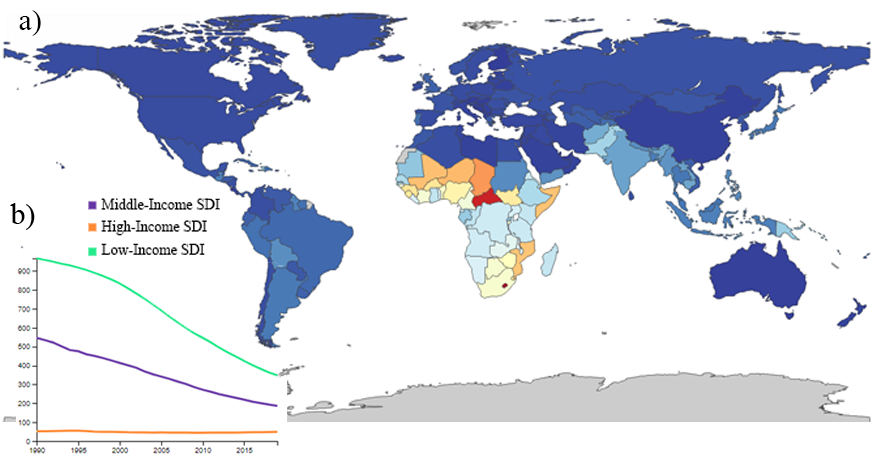
\includegraphics[width=1\textwidth]{figures/Deaths map.png}
    \caption[Summary of world rate deaths burden associated with communicable diseases.]{a) World map representing deaths rate per 100.000 population associated with communicable diseases b) Evolution of the death rate [1990 to 2020]. Adapted from GBD Compare\cite{institute_for_health_metrics_and_evaluation_ihme_uniersity_of_washington_gbd_2015}.}
    \label{fig:Deaths}
\end{figure}
\begin{figure}[b]
    \centering
    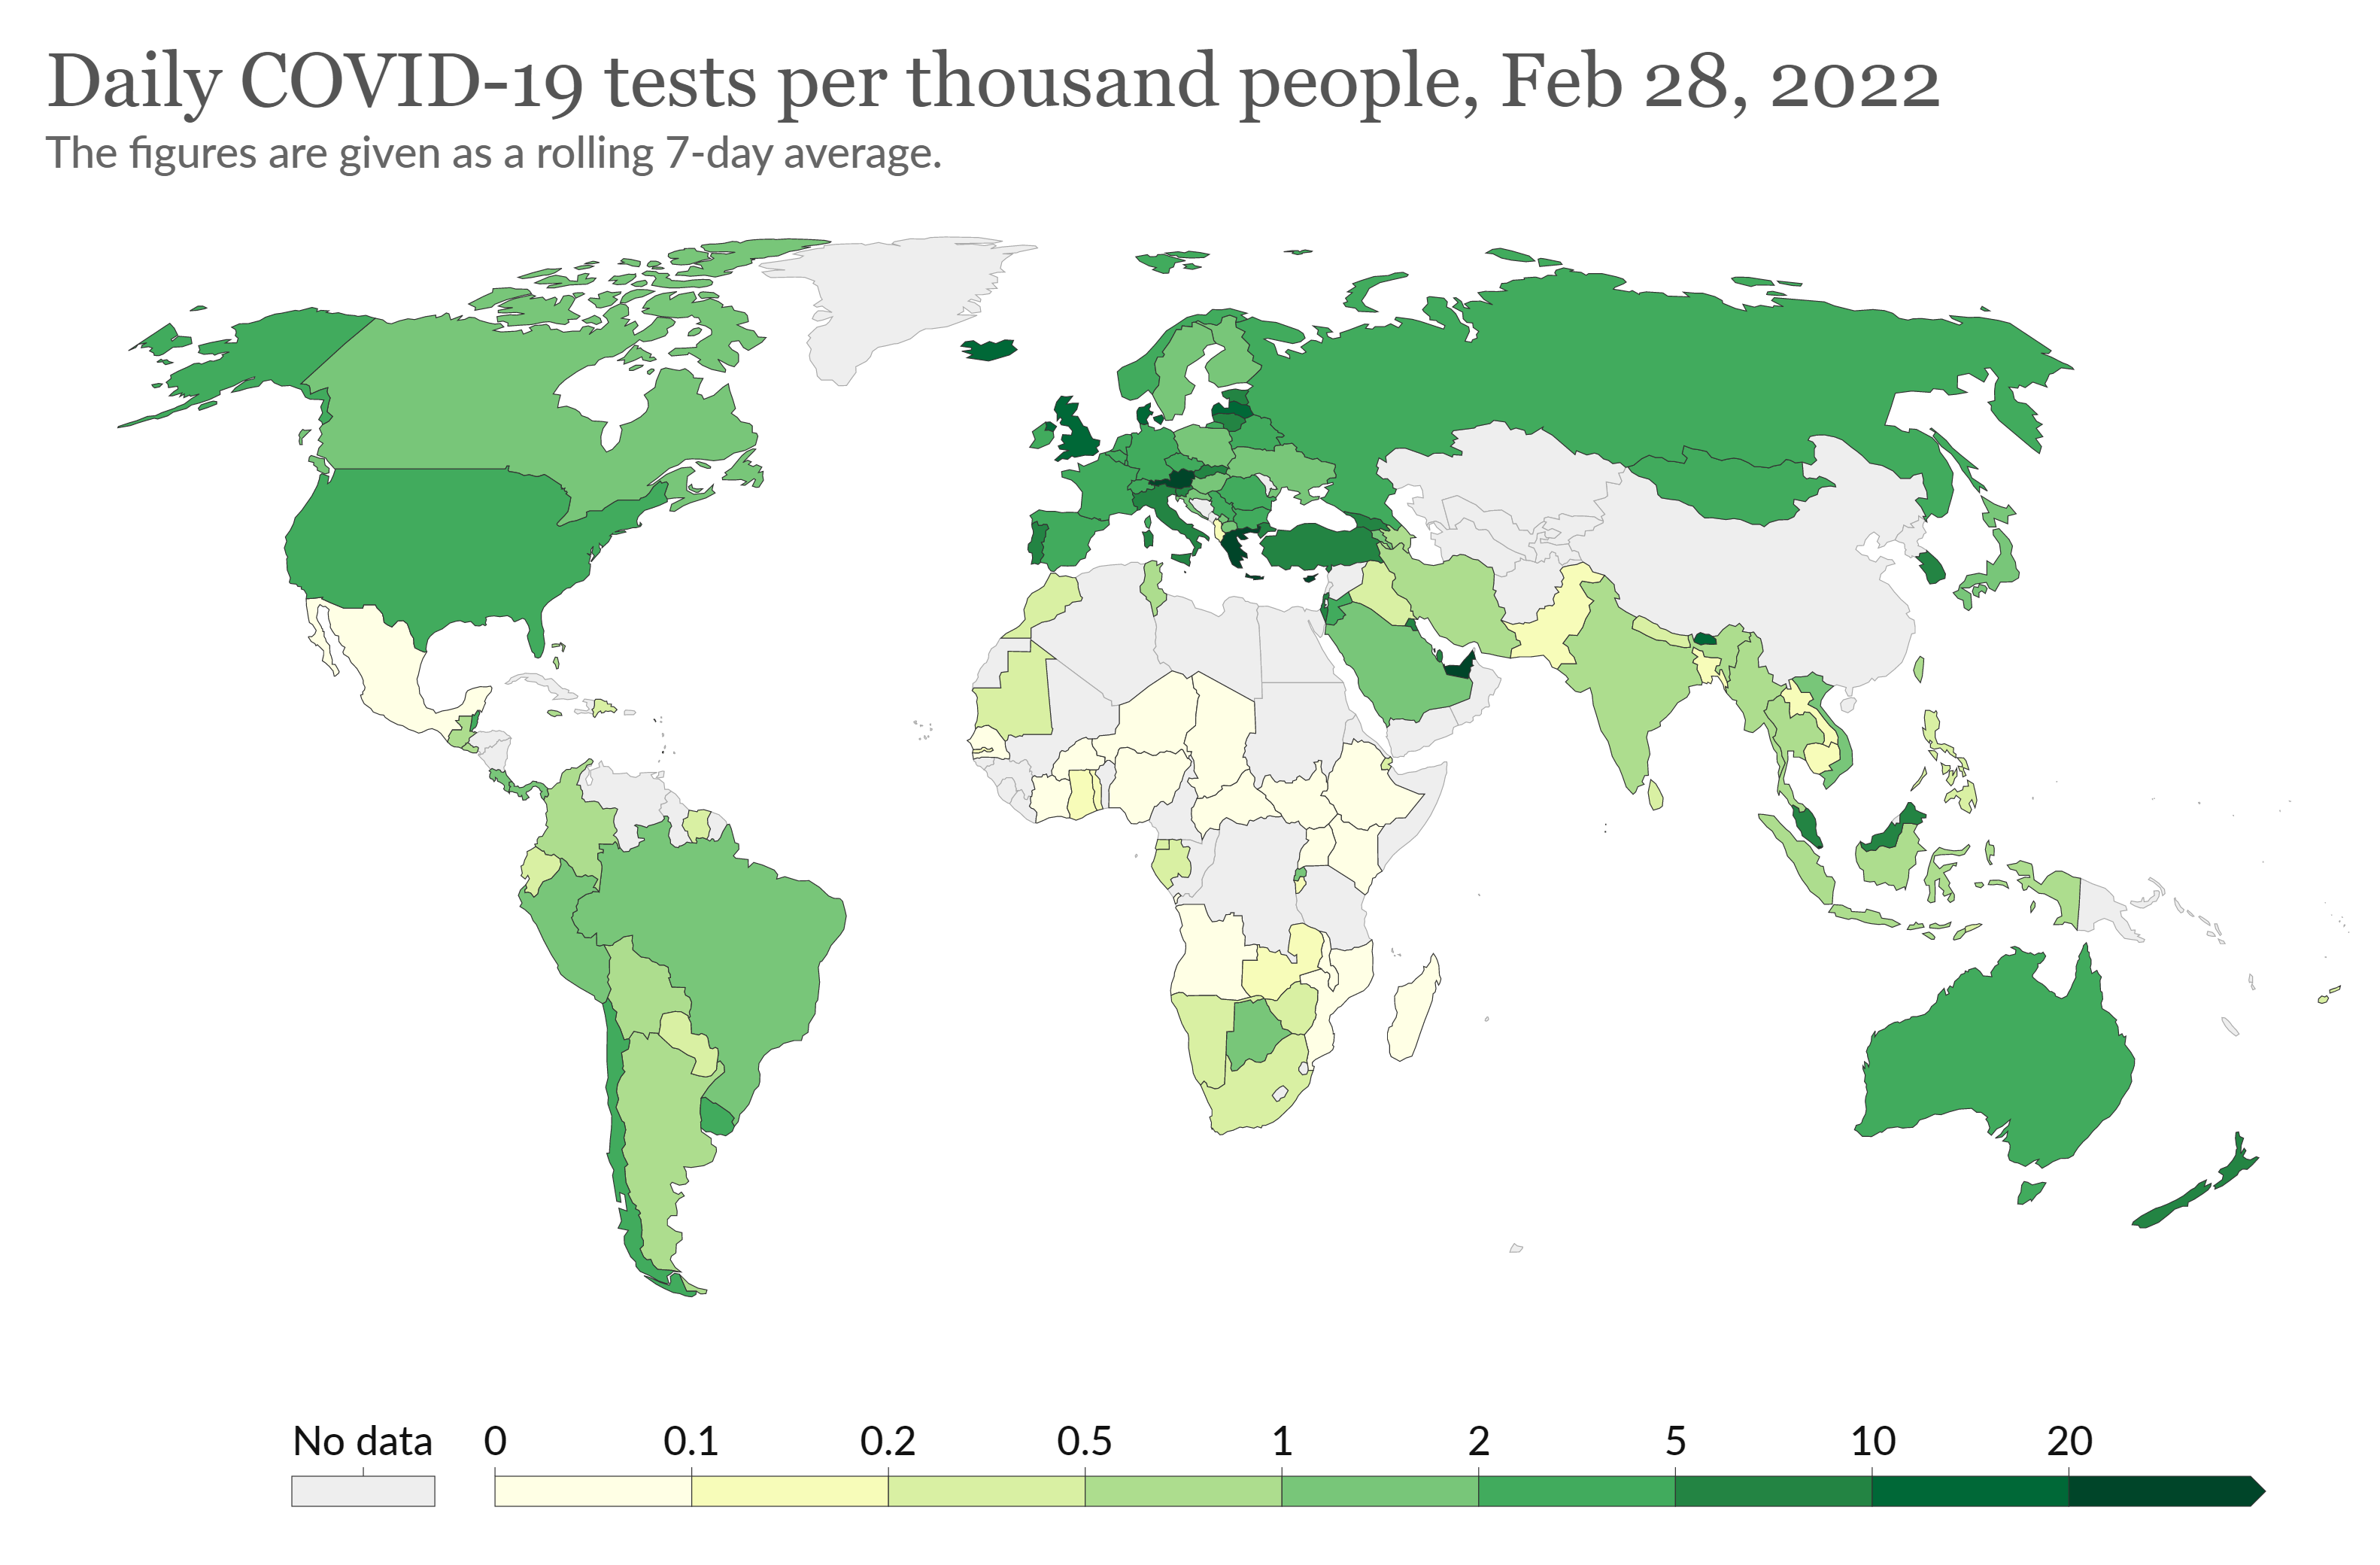
\includegraphics[width=1\textwidth]{figures/diagnosis map.png}
    \caption[World map: total tests performed relative to the size of population.] {World map: total tests performed relative to the size of population. Adapted from Our World In Data\cite{ritchie_coronavirus_2020}.}
    \label{fig:Diagnosis}
\end{figure}
\newpage
\section{Scope of the thesis}
Despite all the challenges faced during the pandemic, I always tried to overcome the problems for staying solid in the original thesis idea. The difficulties that LMICs have always faced to manufacture and deploy diagnosis tests are, since long ago, a meaningful world-challenge at a personal level. In 2019, thanks to my experience coordinating the former Madrid 2019 iGEM team\cite{igem_madrid_2019_aegis_2019}, I had the opportunity to work in Cameroon for a summer, to test our recently developed cholera sensor on the field. During this period, I had the chance to better understand the local communities, their problems and needs. It helped me to deeply interiorize the importance of constructing a world where, starting with healthcare, we all have equally satisfied our basic needs. 

During the SARS-CoV-2 pandemic, as I was not allowed to come back to Tsinghua, I reinvented my thesis plan to adapt it to the new times. I established a collaboration between Tsinghua, Cambridge and Paris universities. In the framework of this collaboration, I travelled to the Centre de Recherches Interdisciplinaires (CRI) in Paris to start using a previous technology I have worked with, QUASR-LAMP, creating a kit that would enable developing regions to perform a high throughput screening on SARS-CoV-2. The idea has always been that, once the pandemic ends, we can adapt these tools  to other communicable diseases for the long-term sake of these regions.

\vspace{12pt}
Following this vision, I defined three main goals for the present thesis:
\vspace{8pt}
\begin{enumerate}
   \item \emph{Adapt the QUASR-LAMP technology to detect the SARS-CoV-2 viral genome.}
   \item \emph{Establish an in-house production of lyophilized reactions that do not require cold chain transportation and storage. Try the system with real clinical samples on the field.}
   \item \emph{Create an affordable hardware that allows incubating and analyzing the results both qualitatively and quantitatively, keeping in mind the resource restrictions of the developing regions.}
\end{enumerate}
%\input{data/Scope}
% !TeX root = ../thuthesis-example.tex

\chapter{论文主要部分的写法}

研究生学位论文撰写,除表达形式上需要符合一定的格式要求外,内容方面上也要遵循一些共性原则。

通常研究生学位论文只能有一个主题(不能是几块工作拼凑在一起),该主题应针对某学科领域中的一个具体问题展开深入、系统的研究,并得出有价值的研究结论。
学位论文的研究主题切忌过大,例如,“中国国有企业改制问题研究”这样的研究主题过大,因为“国企改制”涉及的问题范围太广,很难在一本研究生学位论文中完全研究透彻。



\section{论文的语言及表述}

除国际研究生外,学位论文一律须用汉语书写。
学位论文应当用规范汉字进行撰写,除古汉语研究中涉及的古文字和参考文献中引用的外文文献之外,均采用简体汉字撰写。

国际研究生一般应以中文或英文书写学位论文,格式要求同上。
论文须用中文封面。

研究生学位论文是学术作品,因此其表述要严谨简明,重点突出,专业常识应简写或不写,做到立论正确、数据可靠、说明透彻、推理严谨、文字凝练、层次分明,避免使用文学性质的或带感情色彩的非学术性语言。

论文中如出现一个非通用性的新名词、新术语或新概念,需随即解释清楚。



\section{论文题目的写法}

论文题目应简明扼要地反映论文工作的主要内容,力求精炼、准确,切忌笼统。
论文题目是对研究对象的准确、具体描述,一般要在一定程度上体现研究结论,因此,论文题目不仅应告诉读者这本论文研究了什么问题,更要告诉读者这个研究得出的结论。
例如:“在事实与虚构之间:梅乐、卡彭特、沃尔夫的新闻观”就比“三个美国作家的新闻观研究”更专业、更准确。



\section{摘要的写法}

论文摘要是对论文研究内容的高度概括,应具有独立性和自含性,即应是 一篇简短但意义完整的文章。
通过阅读论文摘要,读者应该能够对论文的研究 方法及结论有一个整体性的了解,因此摘要的写法应力求精确简明。
论文摘要 应包括对问题及研究目的的描述、对使用的方法和研究过程进行的简要介绍、 对研究结论的高度凝练等,重点是结果和结论。

论文摘要切忌写成全文的提纲,尤其要避免“第 1 章……;第 2 章……;……”这样的陈述方式。



\section{引言的写法}

一篇学位论文的引言大致包含如下几个部分:
1、问题的提出;
2、选题背 景及意义;
3、文献综述;
4、研究方法;
5、论文结构安排。
\begin{itemize}
  \item 问题的提出:要清晰地阐述所要研究的问题“是什么”。
    \footnote{选题时切记要有“问题意识”,不要选不是问题的问题来研究。}
  \item 选题背景及意义:论述清楚为什么选择这个题目来研究,即阐述该研究对学科发展的贡献、对国计民生的理论与现实意义等。
  \item 文献综述:对本研究主题范围内的文献进行详尽的综合述评,“述”的同时一定要有“评”,指出现有研究状态,仍存在哪些尚待解决的问题,讲出自己的研究有哪些探索性内容。
  \item 研究方法:讲清论文所使用的学术研究方法。
  \item 论文结构安排:介绍本论文的写作结构安排。
\end{itemize}



\section{正文的写法}

本部分是论文作者的研究内容,不能将他人研究成果不加区分地掺和进来。
已经在引言的文献综述部分讲过的内容,这里不需要再重复。
各章之间要存在有机联系,符合逻辑顺序。



\section{结论的写法}

结论是对论文主要研究结果、论点的提炼与概括,应精炼、准确、完整,使读者看后能全面了解论文的意义、目的和工作内容。
结论是最终的、总体的结论,不是正文各章小结的简单重复。
结论应包括论文的核心观点,主要阐述作者的创造性工作及所取得的研究成果在本领域中的地位、作用和意义,交代研究工作的局限,提出未来工作的意见或建议。
同时,要严格区分自己取得的成果与指导教师及他人的学术成果。

在评价自己的研究工作成果时,要实事求是,除非有足够的证据表明自己的研究是“首次”、“领先”、“填补空白”的,否则应避免使用这些或类似词语。

% !TeX root = ../thuthesis-example.tex

\chapter{Open-Source LAMP hardware}
The previous chapter have described the design and manufacture of freeze-dried QUASR-LAMP reactions allowing the diagnose of SARS-CoV-2 in LMICs. However, as we introduced in the chapter's conclusions, there is still the need for equipment to incubate and analyze the reactions. While incubation requires relatively inexpensive equipment (e.g., a pot and sous vide cooker), the development of the reactions still requires a transilluminator.

Despite previous work by the group to create low-cost transilluminators for GMO detection based in QUASR-LAMP\cite{guy_aidelberg_gmo_2018}, our aim during this thesis was to integrate both the incubation and development equipment into a single unit. For manufacturing the system, we used digital fabrication tools currently spread along the LMIC's maker labs such as Kumasi Hive (Ghana) or the Ongola fab lab (Cameroon).

The second part of this chapter describes the creation of low-cost equipment to carry out Real-Time LAMP experiments, in which the fluorescence generated by the reactions is measured analogically as the incubation progresses. This equipment allows moving forward from qualitative LAMP tests to quantitative measurements (qLAMP), expanding the horizon of possibilities for the assays that can be carried out in remote developing regions.

Both systems are documented in the GitLab of the Open Bioeconomy Lab\cite{francisco_javier_quero_lombardero_open_2021}, an interdisciplinary research group based in the Department of Chemical Engineering and Biotechnology at the University of Cambridge, but also working closely with researchers in Tsinghua University, Cameroon and Ghana. This whole project has been carried out and co-funded as part of OBL, and through its members working on the ground, we have received invaluable feedback and advice.
\newpage

\section{WaterBath}

The idea behind the WaterBath is to serve as a portable and affordable solution to incubate and visualize LAMP amplifications. As it is ideated to work on remote developing regions, the total production price is approximately 5€.

Water is used as the incubating medium because its excellent properties as a thermal conductivity material that makes it a standard in the biotech industry. First, liquid incubation offers higher thermal conductivity than air incubation. Second, from all the materials that keep the liquid state at room temperature, water offers unusually high specific heat capacity, allowing efficient heat transfer over distance with low rates of mass transfer\cite{company_nalco_1979}.

 \begin{figure}[b]
    \centering
    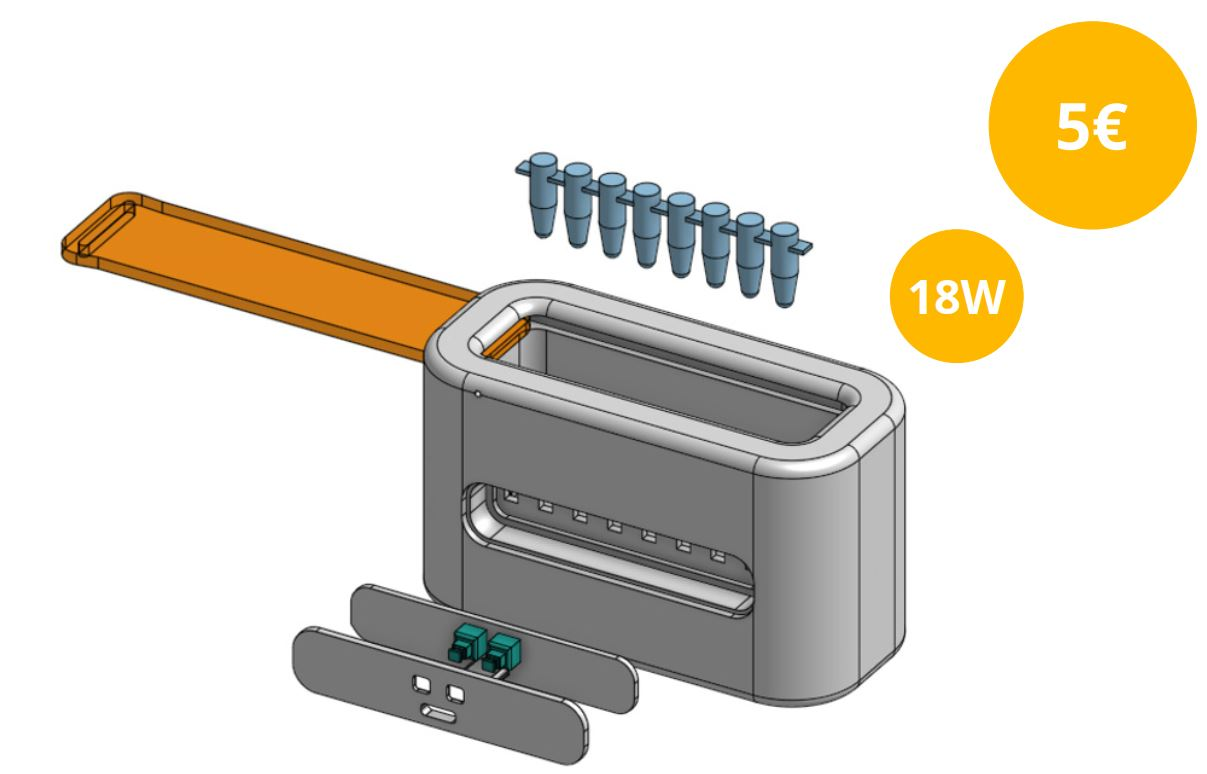
\includegraphics[width=0.95\textwidth]{figures/WaterBath.JPG}
    \caption{Exploded view of the water bath. The system's final price is around 5€ and consumes just 18W, making it possible to power it with an external battery.}
    \label{Exploded view water bath}
\end{figure}

The designed equipment serves as a water bath for incubating the reactions at constant 63ºC, that can be changed by tuning an internal resistor. Following the incubation, the results can be easily analized with an integrated transilluminator made out of 470nm LEDs that light the central chamber from the side, together with a top orange filter that only let go through the green fluorescence of the reactions, filtering out the light from the LEDs. For maintaining the simplicity and the low price of the system, all the electronics are analogic, except the USB-C power deliver negotiator, which allows the system to be supplied by a type C charger able to deliver 9V/12V or even a power bank.

All the designs and manufacturing files can be obtained from the projects' GitLab\cite{francisco_javier_quero_lombardero_open_2021}.


\subsection{Working principle}
The operating mechanism of the water bath is relatively simple; after preparing the QUASR-LAMP reactions, the water bath is filled, closed with the acrylic filter and the incubation button is pressed. A light will turn on while the water bath is heating up. Once the light turn off, the reactions are placed in the eight tube-strips little holders, leaving them incubating for one hour.

Once incubated, the hot water is emptied, and the container is filled with cold water. After waiting 5 minutes for the reactions to cool down (QUASR-LAMP needs to be read cold \cite{ball_quenching_2016}), the second button is pressed, lighting up the side LEDs. This action will illuminate the inner chamber, and the resulting fluorescence will be visible from the top of the water bath if the reactions are positive (Figure 4.2).

 \begin{figure}[b]
    \centering
    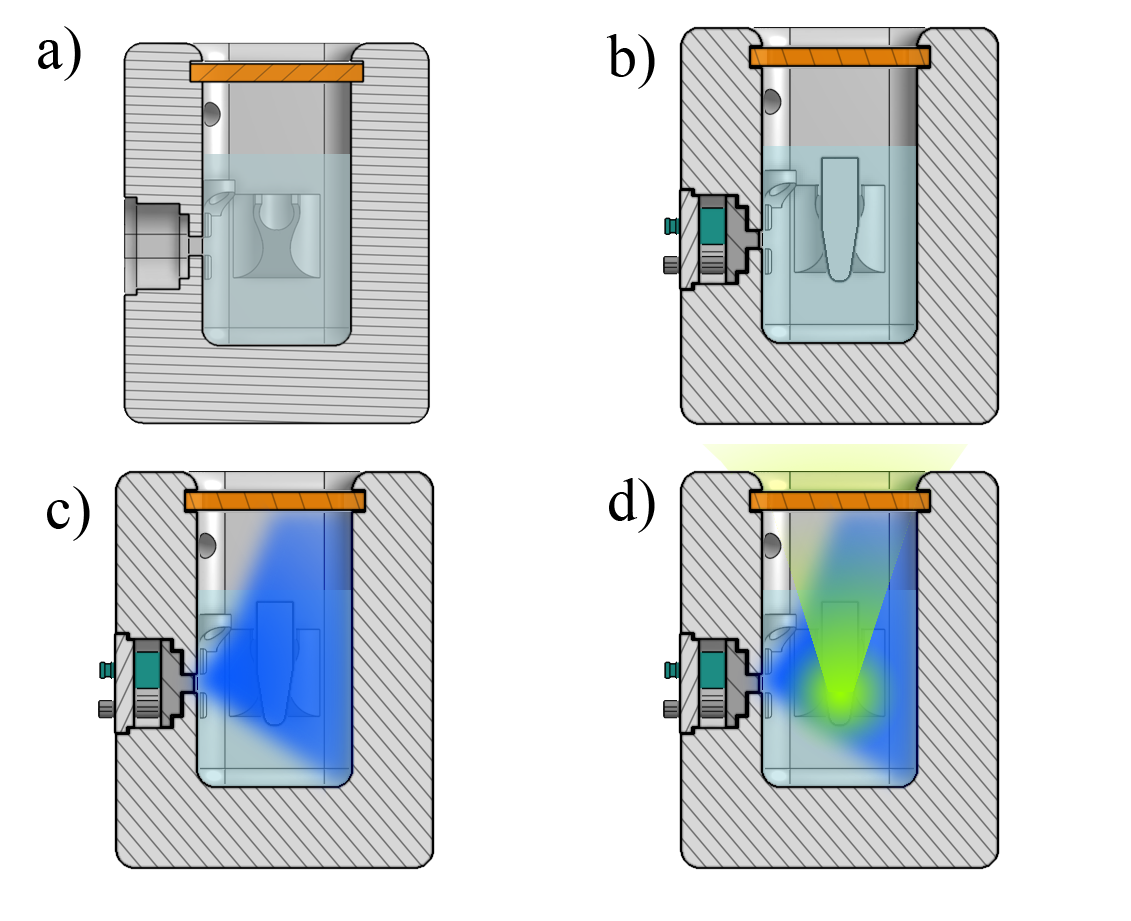
\includegraphics[width=1\textwidth]{figures/WorkingPrinciple.png}
    \caption{Working principle of the water bath. a) The water bath is filled with water, closed and is preheated. b) The reactions are introduced in the holders, and the water bath is closed. c) After one hour, the results are visualized thanks to the activation of the lateral LEDs d) If the reaction is positive, the fluorescence can be observed from the top.}
    \label{Working Principle Water Bath}
\end{figure}

\subsection{Parts}
\subsubsection{Electronics}
The electronics are based on a standard analogue temperature control system, which is robust and straightforward, does not need to be programmed and is exceptionally cheap. It relies on the control of a heater element through a MOSFET regulated by the NE555 chip (Figure 4.3(A)).

The system has been designed for soldering most of the components using the manufacturer's SMT service and parts catalogue (JLCPCB, People's Republic of China), except the USB type C port driver (IP2721\_MAX12), which is readily available from various distributors.

As typically the suppliers only accepts SMT soldering on one side of the PCB, the system has been designed in two parts, which must be separated and soldered back to back. One side consists of the LEDs that illuminate the internal water bath camera, and the other side consists of the rest of the system, the USB connector and the user interface buttons, that faces the exterior of the machine.

The system works with the Type C standard (Figure 4.3 (B)), supporting a 9/12V power supply and allowing the water bath to be plugged on with phone chargers or a power bank capable of supplying these voltages. All schematics and fabrication files can be found on the Open Source Hardware Lab platform\cite{francisco_javier_quero_lombardero_lamp_2021}.

 \begin{figure}[b]
    \centering
    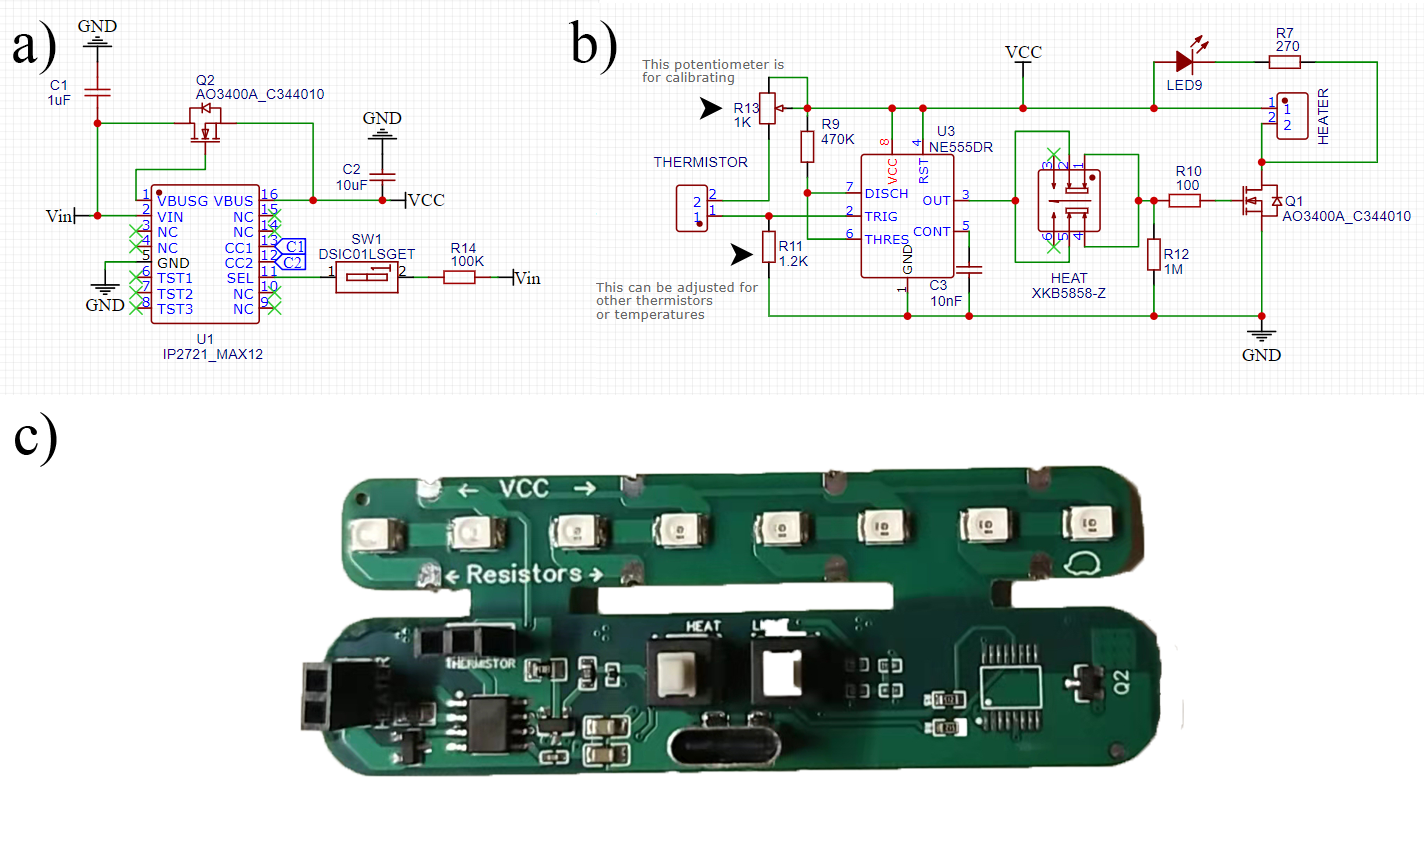
\includegraphics[width=0.9\textwidth]{figures/electronica.png}
    \caption{Schematics of the a) USB C regulator circuit and b) temperature control circuit. c) Printed Circuit Board as it comes from the manufacturer (Without the IP2721 chip). Additional information can be found on the project GitLab\cite{francisco_javier_quero_lombardero_open_2021}.}
    \label{Schematics Water Bath}
\end{figure}

\subsubsection{Case}
The biggest challenge in designing the structure of the water bath lay in the search for affordable materials that stay robust at the temperature at which they needs to work. The primary and most widespread 3D printing technique is Fused Deposition Modeling (FDM) based on melting a plastic filament and then depositing it, with a three-axis motorised system, layer by layer until the final object is created. The major problem with this technique is beside the nature of the materials used. Because they are designed to melt at around 200ºC, they have a glass transition (the temperature at which they begin to deform) of less than half that temperature. Therefore, because 63°C needs to be maintained during the LAMP reaction, most of the traditional FDM materials suffer from deformation, making their use unfeasible.

\begin{figure}[b]
    \centering
    \includegraphics[width=0.65\textwidth]{figures/sla.png}
    \caption{Resulting case from an SLA printing. Model can be found at OnShape platform for SLA\cite{francisco_javier_quero_lombardero_sla_2021} and FDM printing \cite{francisco_javier_quero_lombardero_fdm_2021}.}
    \label{3D printing}
\end{figure}

One possible solution is to employ other printing methods that use non-melting based materials. One such technique is stereolithography 3D printing (SLA). This technique uses resins that polymerise due to exposure to light, typically consisting on blue or shorter wavelengths. SLA printing equipment uses a laser beam to polymerise the final part layer by layer inside a tank. We experimented with creating the case employing a Formlabs SLA printer (and their compatible resin) with a satisfactory result (Figure 4.4). Unfortunately, although we modified the 3D model to be hollow and use less material\cite{francisco_javier_quero_lombardero_sla_2021}, the price of the Formlabs resin is still too elevated for this application, resulting in a part costing more than 10€.


Although a possible solution is to go to lower-cost SLA printing brands (e.g. Creality or Anycubic), another restricting factor relies on the fact that this 3D printing technology is less widespread in maker labs, especially in developing countries. For this reason, we experimented with FDM printing materials that have a glass-transition temperature above 80ºC. One such material is PETG, which in practice gave us good results. Furthermore, the prices of printing the case with PETG are less than a \$1. Models for FDM 3D printing can be found on the OnShape platform\cite{francisco_javier_quero_lombardero_fdm_2021}.

\subsubsection{Heater design}
Aiming to find a solution that adapts to our needs in terms of power consumption, shape and price, a custom made PCB heater was designed. The heater shape was derived from the bottom of the waterbath and the trace width and length was calculated using the following formula:


\begin{equation*}
\centering
R = \rho \cdot \frac{L}{T \cdot W} \cdot [1 + \alpha (temp -25)]
\end{equation*}
\vspace{12pt}
\begin{center}
    \small{\textbf{Where:} $R$ = resistance, $ρ$ = resistivity, $L$ = length, $T$ = trace height, $W$ = trace width, \\$α$ = temperature coefficient, $temp$ = temperature}
\end{center}
\vspace{12pt}

We calculate the trace to consume around 1.5 A at 12V and 60ºC. The resulting resistance is 8Ohm with a length of 217cm and a width of 0.16mm. The PCB was manufactured using aluminium as the support (JLCPCB, People's Republic of China). In the heat uniformity analysis the PCB heater performed well, with less than one degree of difference between the perimeter and the center (Figure 4.5). All schematics and fabrication files for the heater can be found on the Open Source Hardware Lab platform\cite{francisco_javier_quero_lombardero_lamp_2021}.

\begin{figure}[b]
    \centering
    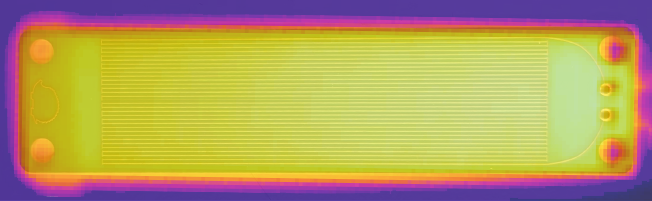
\includegraphics[width=0.7\textwidth]{figures/heat uniform.png}
    \caption{Heat uniformity analysis of the designed heater.}
    \label{Heat uniformity}
\end{figure}
\newpage

\subsubsection{Optics}
The optics of the water bath are based in three main components (Figure 4.6):
\begin{itemize}
\item The light source, consisting of a 470nm LED (Mouser Electronics, UK).
\item The QUASR-LAMP probes containing fluorescein, a fluorophore that absorbs at the blue wavelength of the source and emits in a green one.
\item The filter at the top of the water bath, which allows only the green light to pass through, separating the fluorophore's emission from the light source. 
\end{itemize}
\vspace{12pt}
\begin{figure}[h]
    \centering
    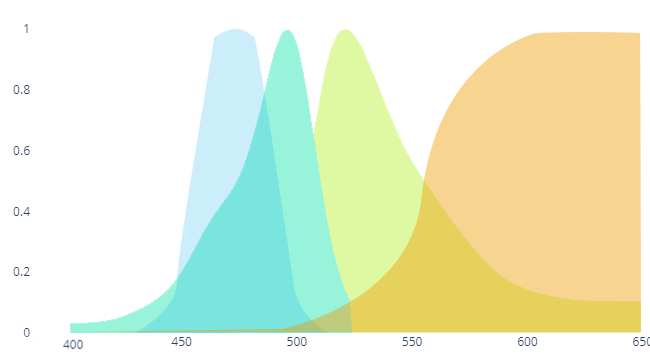
\includegraphics[width=0.8\textwidth]{figures/wavelengths.png}
    \caption{Spectrum from the different components of the optic system. \textcolor{blue}{Blue}, LED emission; \textcolor{Turquoise}{Turquoise}, Fluorescein absorbance; \textcolor{GreenYellow}{Green}, fluorescein emission; \textcolor{Orange}{Orange}, spectrum allowed by filter.}
    \label{wavelengths}
\end{figure}
\vspace{12pt}

Different solutions were explored to solve the challenge of finding an affordable filter with good performance. Firstly, filters from a manufacturer of theatrical lighting products (LeeFilters, UK) were explored. The manufacturer was chosen because of their vast range of filters, the excellent price (at a few euros per $m^2$) and outstanding characterisation of their absorption spectrum. The filters were mounted on a 3D printed holder that fitted into the top slot of the WaterBath (Figure 4.7(A)). The main issue we faced with this system is their tedious fabrication and the fragility of the result. For this reason, we found a better solution cutting the entire filter out of a piece of 3mm thick transparent orange acrylic (Figure 4.7 (B)).

\begin{figure}[h]
    \centering
    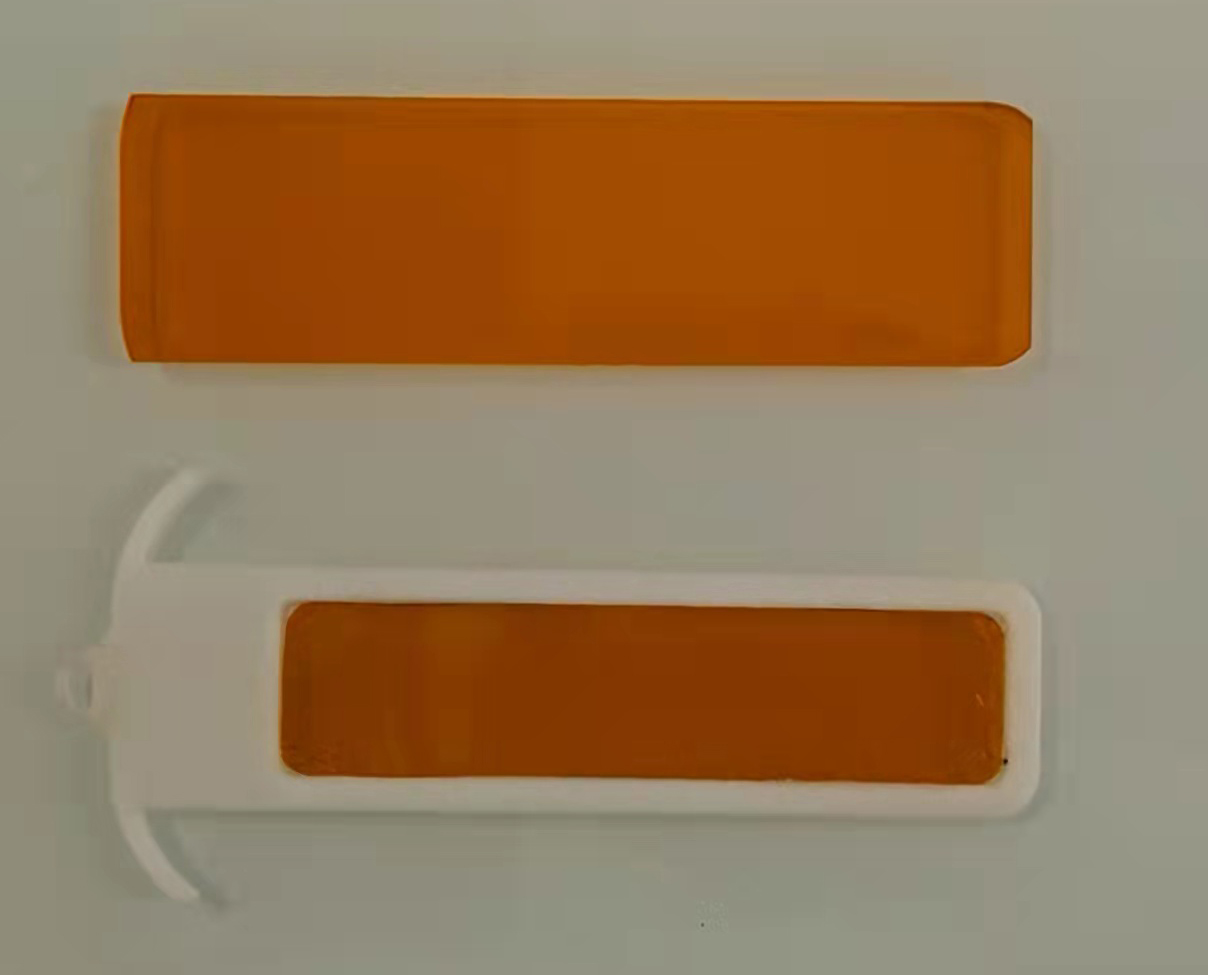
\includegraphics[width=0.8\textwidth]{figures/filters.jpg}
    \caption{The two solutions used as a filter for the waterbath. At the top is a filter cut entirely from transparent orange acrylic. At the bottom is a low-cost filter for theatrical lighting (LeeFilters, UK) on a 3D printed support.}
    \label{filter}
\end{figure}

\newpage
\subsection{Results and conclusions}
The water bath was benchmarked against the combination of a thermocycler (BioRad, US) and a low-cost transilluminator (IORodeo, US), comparing their performances to incubate and analyze QUASR-LAMP reactions (Figure 4.8). Combined with Corona Detective reactions, both systems showed a detection limit of one viral copy per uL. These results demonstrate the ability of the kit to detect coronaviruses at a meagre cost, with a water bath of \$5 and reactions of less than \$2. Furthermore, the system is portable and can be supplied by a power bank battery. However, more results are needed to characterize the number of reactions per charge. 

As a final point, the hardware has been conceived and designed to be replicated in locally by the use of inexpensive digital manufacturing techniques. We are working with the maker labs near our collaborators in LMICs to try to replicate the system on the field and collect feedback on usability for future versions.

\newpage
\null
\vfill
\begin{figure}[h]
    \centering
    \includegraphics[width=0.95\textwidth,keepaspectratio]{figures/waterbath results.png}
    \caption{(Top-left) Results of Corona Detective amplification testing the water bath. (top-right) Comparison of the amplification results between the water bath and a commercial thermocycler employing an external transilluminator. Both results show equivalent, with a detection limit of 20 copies per reaction (~1 viral copy per microlitre). (Bottom) Image depicting the reaction preparation process prior to incubation.}
    \label{wb results}
\end{figure}
\vfill


\newpage

\section{Real time LAMP equipment}
As mentioned in the first chapter, Real-Time PCR is the current gold standard in the diagnosis field. Reading the fluorescent signal constantly at each amplification cycle is the essential characteristic of this technique, allowing the kinetics of the reaction to be observed in detail. The advantages of this technique compared to end-point reactions are numerous. First of all, the real-time measurement allows catching false positives that may have been generated in the last moments of the reaction due to aberrant amplification (Figure 4.9). Secondly, it makes possible the optimisation of the different features of a reaction (different primer sets and their ratios or enzyme and magnesium concentrations, among others) since it offers the opportunity to compare precisely the different performances associated with the combinations of the features.

\begin{figure}[b]
    \centering
    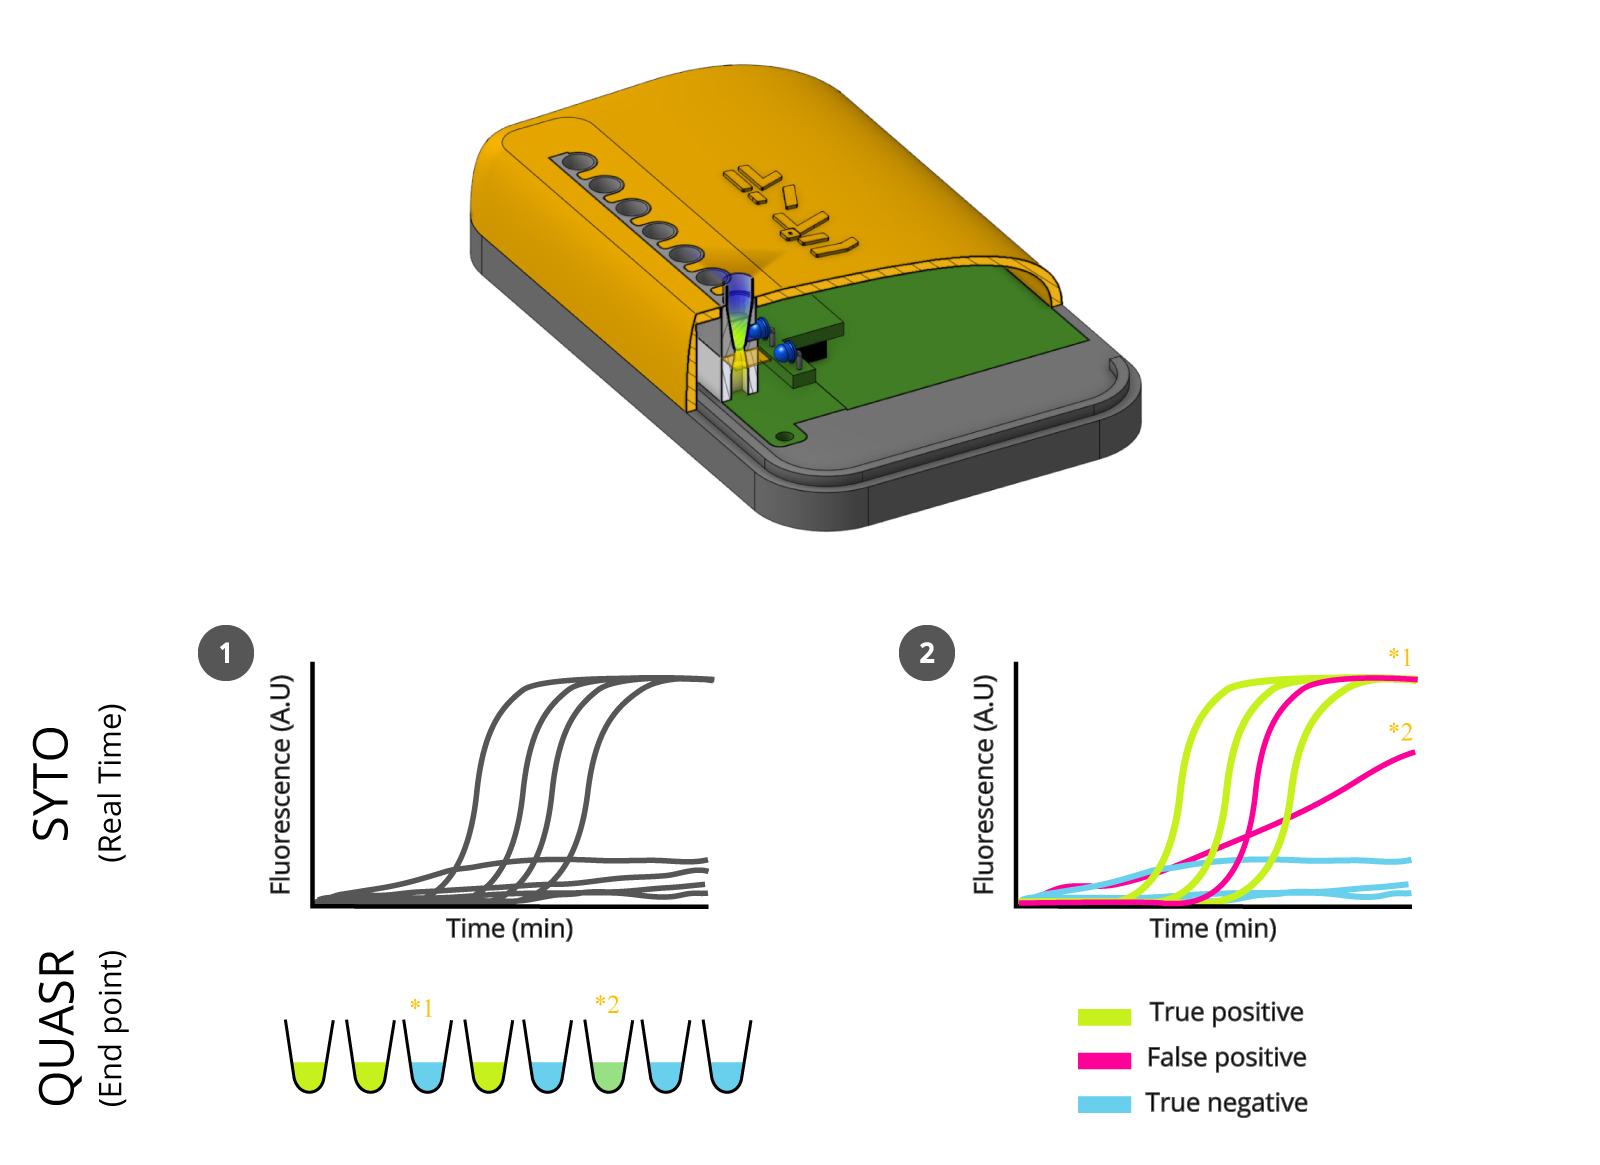
\includegraphics[width=0.95\textwidth,keepaspectratio]{figures/qlamp.png}
    \caption{(Top) Section of the Real-Time LAMP machine. (Bottom) Detailed process of false-positive filtering using real-time QUASR amplification. (1) Reactions are amplified, measuring SYTO9/82 fluorescence in real-time and cooling down the reactions to obtain an end-point value of the QUASR fluorescence. (2) The unspecific amplifications, spotted thanks to the end-point result of the QUASR detection and the real time measurements, are filtered from the real-time amplification data.}
    \label{qLAMP}
\end{figure}

The fundamental problem of Real Time PCR technique is the expense of the equipment. If a normal thermocycler costs around \$3000, a qPCR machine costs in the order of magnitude of \$30.000, which is prohibitively expensive in areas where even a stable electricity supply is not assured. During this thesis, the last goal to address has been to develop a machine that allows real-time quantification of isothermal amplification in real-time, affordably and straightforwardly, to ultimately enable remote low resource areas to perform quantitative nucleic acid testing. 

The development of this equipment is still in progress, so the results of this thesis are preliminary, and the scientific publication in which they will be included is in preparation. 


\subsection{Design}

The equipment is divided into six subsystems (Figure 4.10):

\begin{itemize}
\item \textbf{The microcontroller module}, consisting of an ESP32 that allows control of the machine through the local network, acting as a server and allowing the end-user to interact with the system through a simple web page. 
\item \textbf{The lighting module}, consisting of 8 blue LEDs emitting at 470nm and governed by a standard LED driver in the maker ecosystem (WS2814, WorldSemi).
\item \textbf{The fluorescence readout module}, consisting of a photodiode, a transimpedance amplifier circuit and a dedicated 16-bit analogue-to-digital converter. Prior to signal measurement, the light is filtered with a LeeFilter number 105. 
\item \textbf{The incubation module}, governed by a Proportional-Integral-Derivative (PID) algorithm that activates a Kapton-based heating element. The heating element is sticked to a 3D printed aluminium piece (Jiinsoon LTC, People's Republic of China) that holds the 8-tube strips with the reactions and channels the resulting fluorescence to the light-sensing module.
\item \textbf{The power supply module}, similar to the one previusly described in the water bath section. It is based on the USB type C standard and allows the user to power the entire device with a phone charger or even a power bank.
\item \textbf{The housing case}, 3D printed on PETG using an FDM printer (Prusa i3, Prusa Research).
\end{itemize}

All the detailed schematics, manufacturing files and 3D models can be found in the GitLab page of the project \cite{francisco_javier_quero_lombardero_open_2021}.

\newpage
\null
\vfill
\begin{figure}[h]
    \centering
    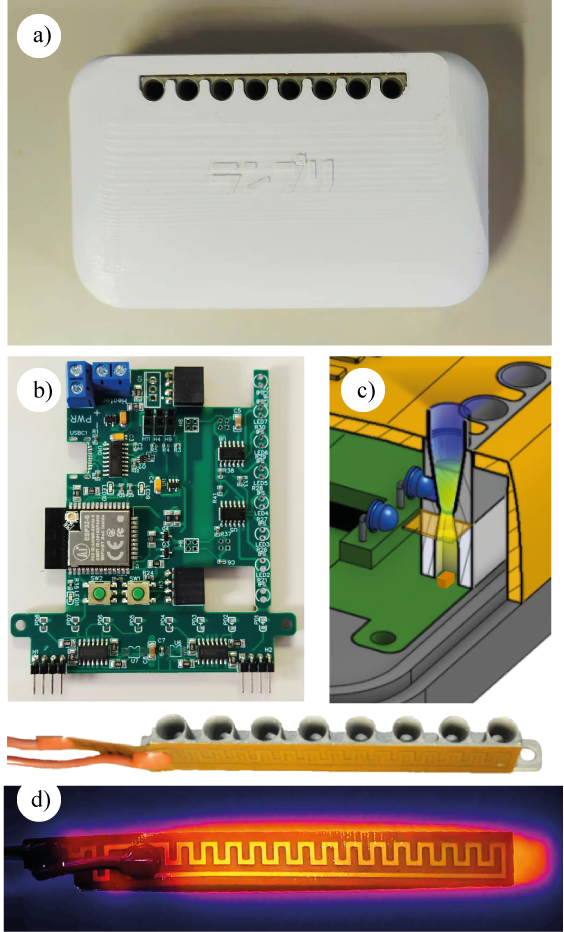
\includegraphics[width=0.55\textwidth,keepaspectratio]{figures/qLAMP-parts.png}
    \caption{Detail of the Real-Time LAMP machine modules. (a) Case of the machine 3D printed in PETG. (b) Detail of the electronics. The PCBs from the different modules come together, so they need to be broken apart and joined using the connectors. The ESP32 microcontroller governs all the modules and connects the machine to the local network, allowing the user to control the machine and see the results in real-time through a phone or a computer connected to the same local network. (c) Detail of the optics module. The LEDs light the reaction tubes from the side. If the reaction is positive, and therefore fluorescence is generated, the light goes down through a hole in the metal piece, crosses the high pass filter, and reach the photodiodes in the sensor PCB below the holder. (d) Detail of the metal holder with the Kapton heater stuck in the back (Top). Heating uniformity analysis of the Kapton heater (Bottom). All the electronic schematics and 3D models can be obtained from the Gitlab repository of the project\cite{francisco_javier_quero_lombardero_open_2021}.}
    \label{qLamp parts}
\end{figure}
\vfill


\newpage

\newpage
\subsection{Results and conclusions}
As previously introduced, this equipment is still under development, and therefore the results are preliminary. Therefore, they should be understood as a first sample of the system's future potential and not as a final result. 

A simple assay was performed using SYTO9 as the signal generator to test the system's ability to measure the amplification in real-time (Figure 4.11). Despite preliminary results showing a sensitivity with a vast margin for improvement, the system successfully measured the signal in real-time in this first test. This data indicates that the prototype is on track to become a real-time LAMP machine successfully. However, this results evidenciate the need for further work after this thesis, to reduce noise, increase sensitivity, and benchmark the system against the RT-PCR gold standard.   

\begin{figure}[b]
    \centering
    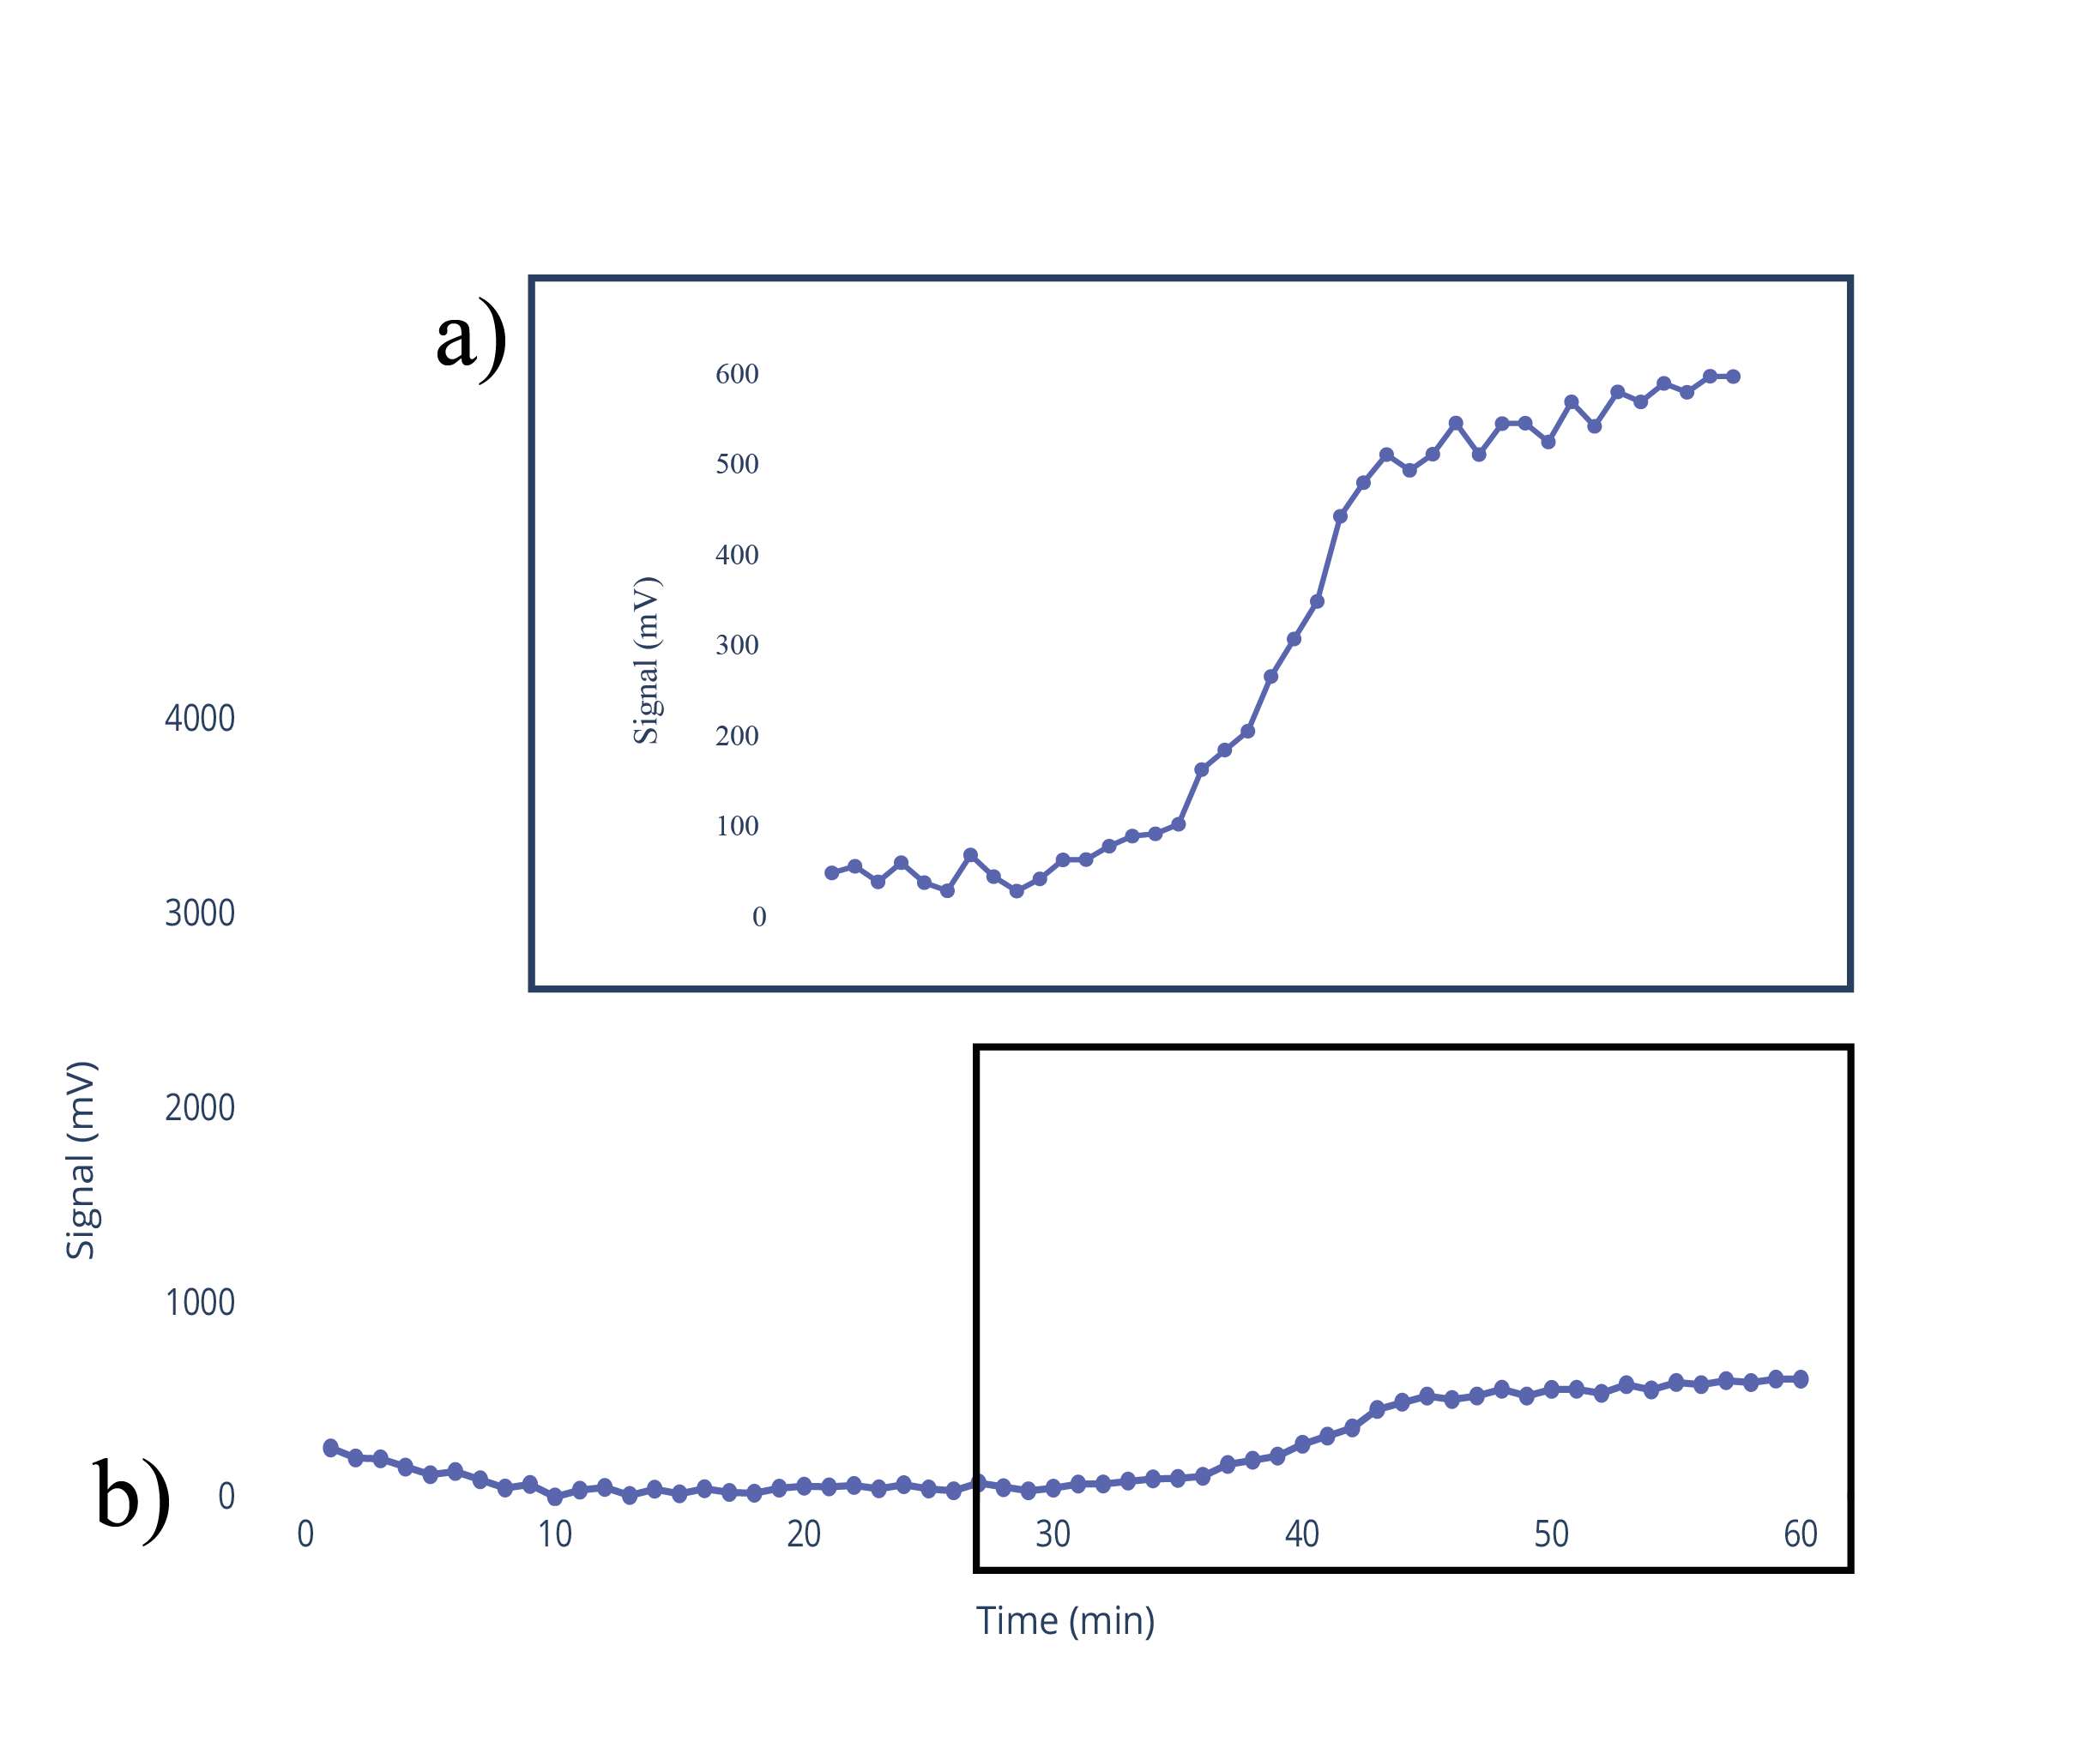
\includegraphics[width=0.9\textwidth]{figures/signal.png}
    \caption{Although the signal can be distinguished in a real time amplification-like result (a) the signal is still small compared with the entire range of the system (b). This results evidenced the need of continuing experimenting with solutions that helps increasing the signal.}
    \label{qLAMP signal}
\end{figure}

The total price of manufacturing the system on a small scale (using digital manufacturing techniques) is broken down in Table 4.1. It should be noted that the price of the system is about 3 orders of magnitude lower than a commercial Real Time PCR machine.

\begin{table}[]
\centering
\begin{tabular}{rl}
\textbf{Component}    & \textbf{Price (USD)} \\
Assembled electronics & 45                   \\
3D printed alluminium tube holder           & 7                    \\
3D printed printed case      & 1                    \\
Kapton heater         & 1                    \\
Optic filter          & \textless{}1         \\
\textbf{Total}        & \textbf{54}         
\end{tabular}
\caption{Breakdown of manufacturing prices.}
\end{table}


It is also important to mention that, for performing real-time measurements, the QUASR-LAMP technology presents a critical problem; the fluorescence needs to be read in cold or, at least, at room temperature. As mentioned in the first chapter, in QUASR-LAMP the quencher-fluorophore combo is designed with a melting temperature significantly lower than the incubation temperature, aiming that the quencher probe does not compete for the primer during the reaction. Because of that, measuring the fluorescence at room temperature involves thermocycling between the incubation temperature (63°C) and room temperature. This process is tantamount to missing the main advantage of isothermal amplification, the no requirement of thermal cycling, making the system more complex, expensive, and less portable. To overcome this challenge, we found two possible alternatives to measure a specific LAMP amplification in real-time.

The first solution comes hand in hand with the use of DARQ technology, similar to QUASR but with a fluorophore/quenching probe melting temperature similar to the rest of the primer set, and therefore generating the fluorescence at then incubation temperature. As mentioned previously, this will generate the quenching probe to compete for the primers with the target, slowing down the speed of the reaction.

The second possible solution, may be to include in the QUASR-LAMP mixture an intercalating agent such as SYTO9/82, hot-readable and described as non-inhibiting amplification\cite{oscorbin_comparison_2016}. This procedure allows a real-time amplification signal to be obtained thanks to the intercalating agent and, subsequently, to cool the reaction and filter out false positives with the specific end-point signal generated by QUASR (Figure 4.9). 

Both solutions need to be further explored in the future, as having reach this point the time and resources available in the framework  of this thesis came to an end.

% !TeX root = ../thuthesis-example.tex

\chapter{Discussion and future perspectives}

\begin{figure}[b]
    \centering
    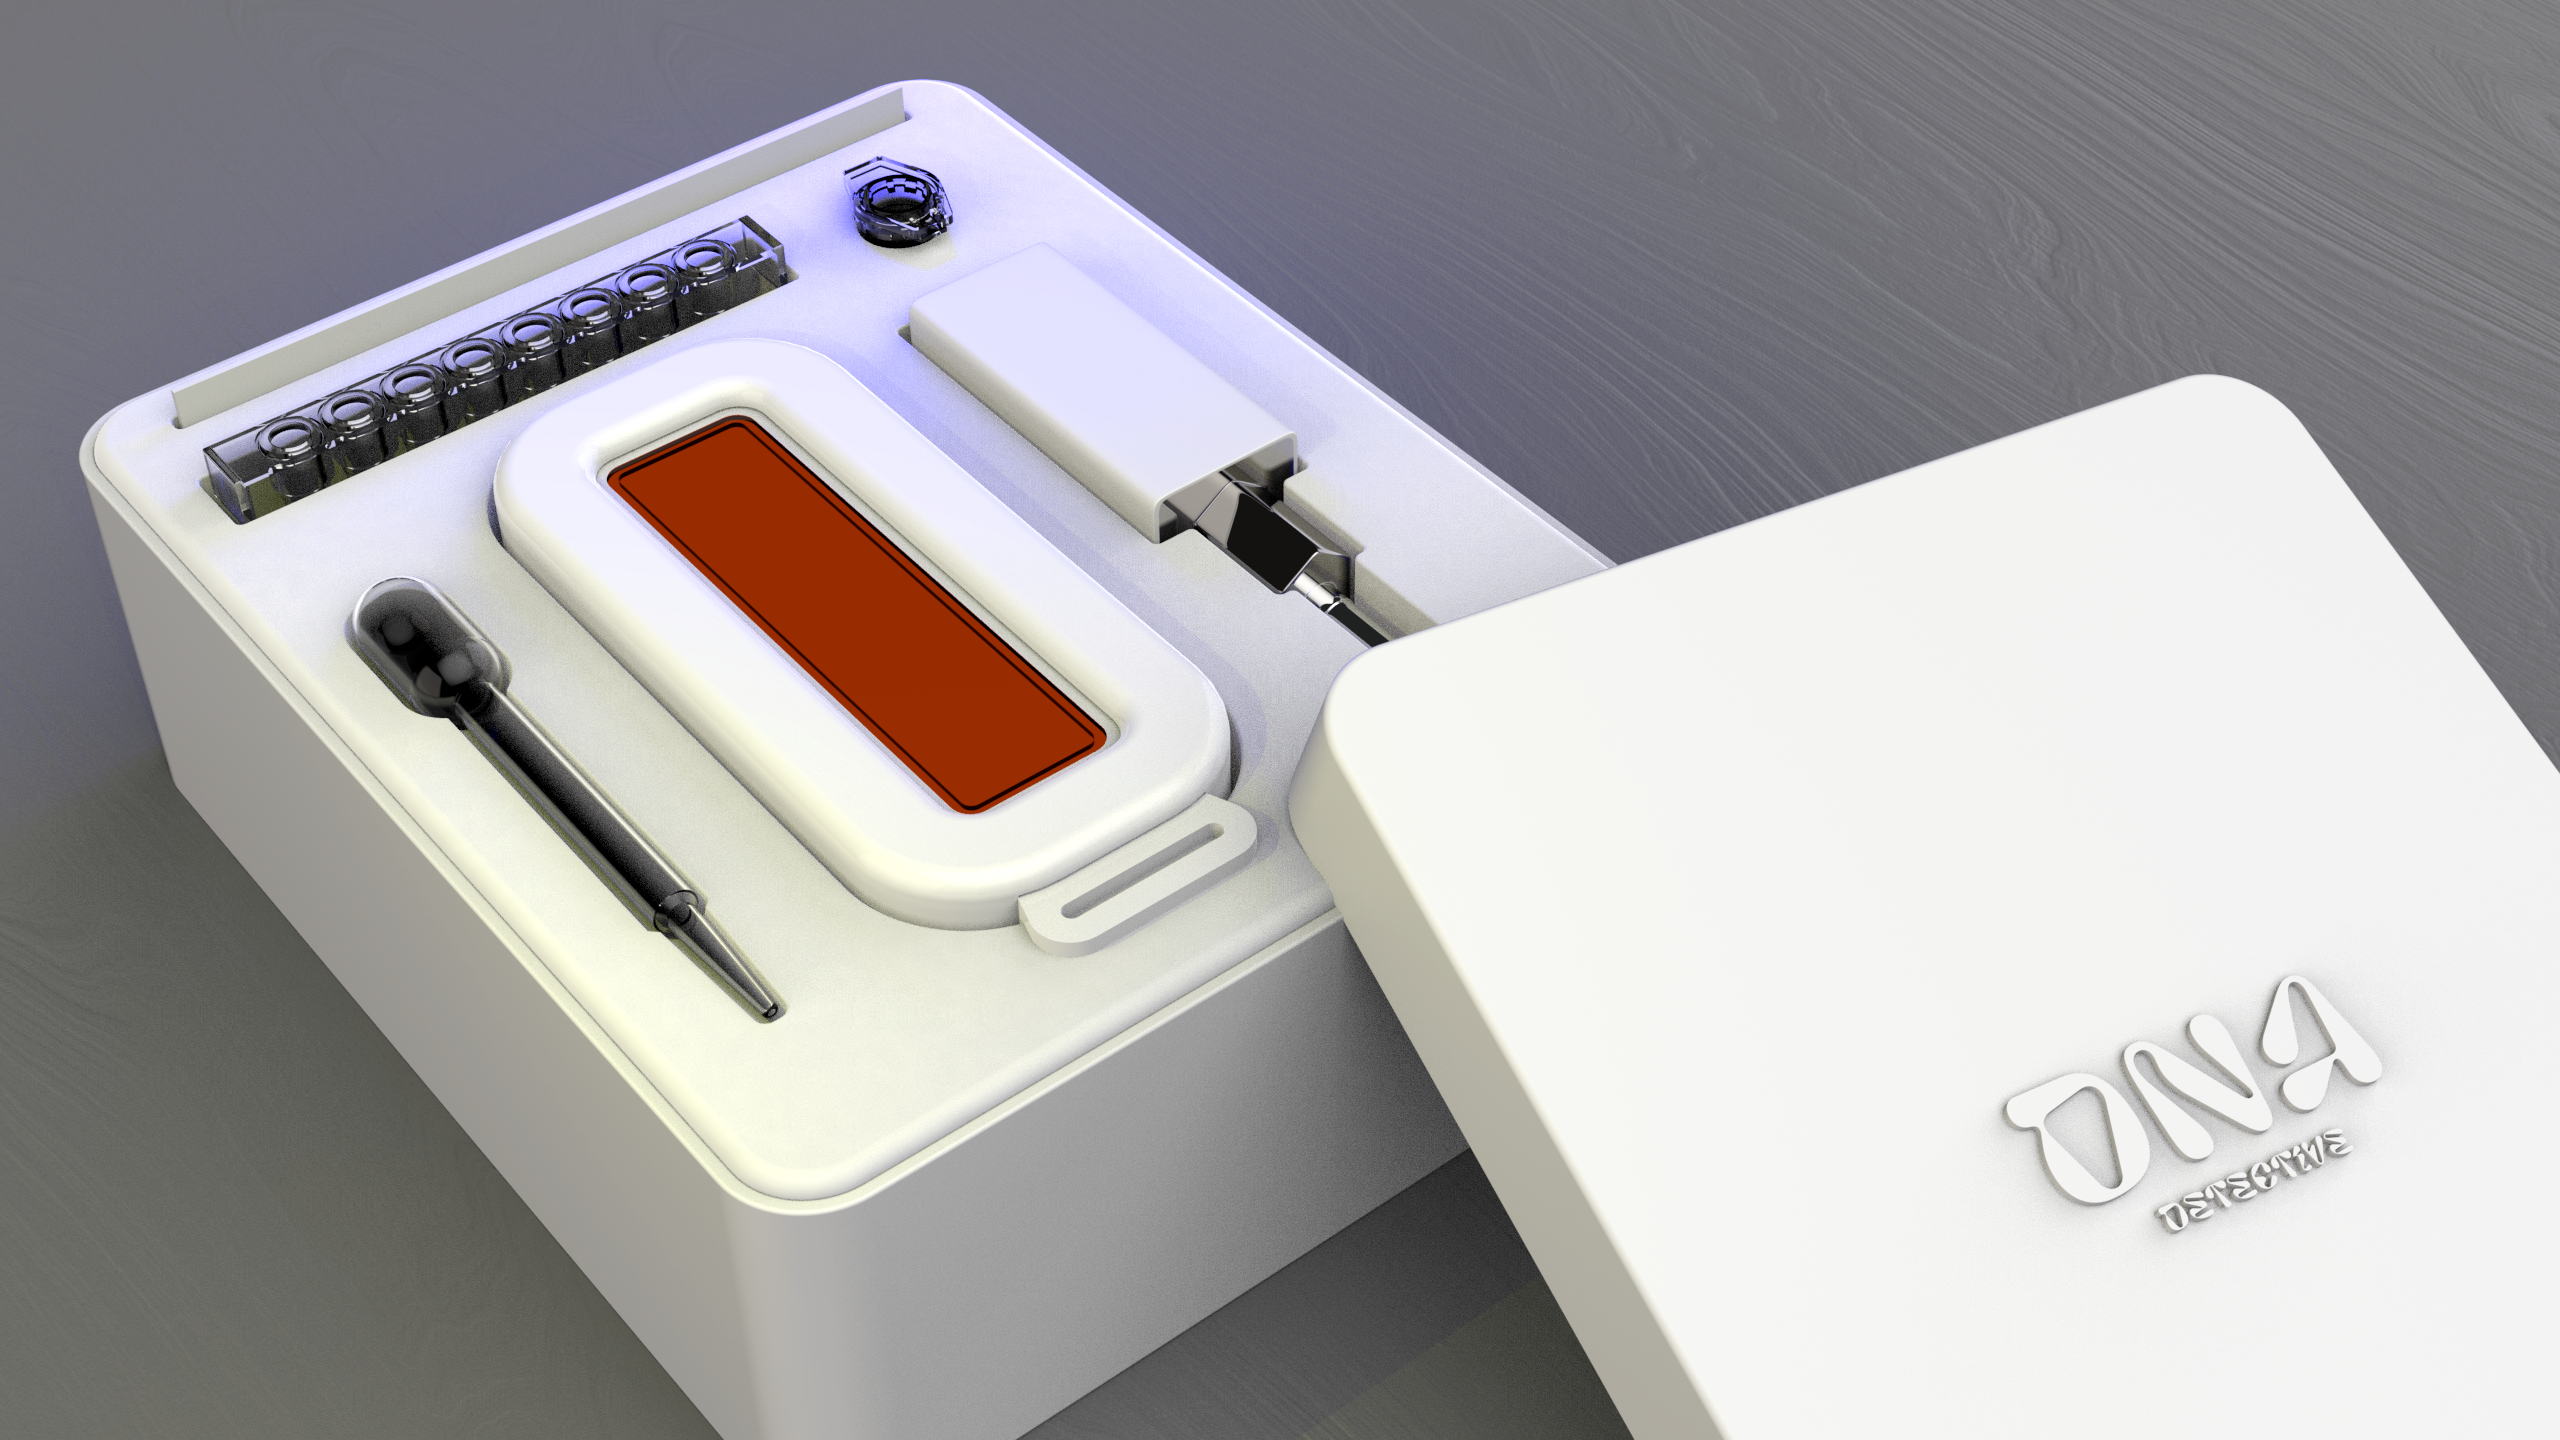
\includegraphics[width=0.95\textwidth]{figures/kit simulation.png}
    \caption{Simulation of the final kit. Image generated by Blender using the 3D models in the GitLab repository of this project\cite{francisco_javier_quero_lombardero_open_2021}.}
    \label{Final kit}
\end{figure}

During this thesis, we have described the design and successful implementation of a series of biotechnological and hardware tools that take the simplicity and affordability of infectious disease detection to the next level. In addition, both protocols and designs have been registered under open source licenses, allowing anyone to replicate the system locally.
    
Although future additional tests are needed (with better quality clinical samples) the performance of both CoronaDetective and water bath reactions has been satisfactorily demonstrated throughout this thesis. Furthermore, the possibility of lyophilizing the reactions to vastly increase their room temperature stability has been described. With a price of \$2 for the reactions and \$5 for the hardware, being easy to use and replicate, not needing refrigeration, being portable and presenting the robustness to false positives of a PCR, this technology presents itself with a great potential to be a game-changer in the low resource diagnostics panorama.
 
 \newpage   
The real-time lamp kit described in the last part of Chapter 4, while still requiring future adjustments, has enormous potential to enable the quantitative analysis of nucleic acid amplification at the price of ~\$50. This cost represents three orders of magnitude of improvement over previous commercial alternatives and opens a massive window of possibilities for both research and diagnostics in LMICs.

However, future work is still needed. To achieve a real impact, we must gain recognition for the use of this technology as an \emph{in vitro} diagnosis certified tool. In this topic, we have an advanced conversation with the local regulatory agencies in Ghana, the Noguchi institute and the local Ghana FDA agency. In our opinion, the next important step on the road to certifying and deploying the technology involves creating a kit in the form of a final product containing all the components necessary to carry out the detection protocol. This kit should package inside the hardware, reactions, and other materials an end-user requires, such as affordable liquid handling solutions or a simple and intuitive user manual (Figure 5.1). Once an initial batch of the kit is produced the system will be ready to enter in the trials to get the local \emph{in vitro} diagnosis certification.
        
Nevertheless, the largest potential to support the development of LMICS is stablishing a local production of the technology. The reactions are simple, using a single enzyme, which is crucial in making production possible in the field. Early in the pandemic, we contributed to create the Reclone online collaborative network \cite{recloneorg_reagent_nodate} in which researchers around the world can share and review protocols for enzyme production at low resources settings. To start exploring the local production of enzymes, many researchers have been exploring ways of harvesting the potential of synthetic biology to create easy protocols to produce and purify Bst polymerases on the field\cite{rivera_recombinant_2020}. If Bst can potentially be manufactured on the ground, this would allow LMICs to gain enormous industrial autonomy from the main producing areas of the planet (Europe, the United States and China), alleviating the bottlenecks generated by the dominant centralized manufacturing model.
        
Following the same principle, the hardware has been designed to be partially manufactured using digital fabrication techniques spread across any region of our planet. The only component that remains difficult to manufacture entirely in the field are the electronics, but they have been designed in such a way that their complete assembly can be outsourced to the big production facilities of production hubs as Shenzhen, from where they can be shipped to the destination countries for further local assembly with the rest of the parts.
        
This process will help improve the supply chain and combat bottlenecks in the deployment of these technologies on the ground and, in the long run, will have a positive impact on industrially upgrading these countries. It is because of this that the development and application of these types of frugal technologies have a much broader impact than only in the diagnostics field, being also able to accelerate the industrial development of remote regions by facilitating the transition to a local production of diagnostic technologies.
        
We believe that the future is open source, as only through collaboration we can overcome the greatest challenge of this century and build a world worth living in.
        
        
        
        




% 其他部分
\backmatter

% 参考文献
\bibliography{ref/zotero}  % 参考文献使用 BibTeX 编译
% \printbibliography       % 参考文献使用 BibLaTeX 编译

% 附录
% 本科生需要将附录放到声明之后,个人简历之前
\appendix
% % !TeX root = ../thuthesis-example.tex

\begin{survey}
\label{cha:survey}

\title{Title of the Survey}
\maketitle


\tableofcontents


本科生的外文资料调研阅读报告。


\section{Figures and Tables}

\subsection{Figures}

An example figure in appendix (Figure~\ref{fig:appendix-survey-figure}).

\begin{figure}
  \centering
  
\includegraphics[width=0.6\linewidth]{example-image-a.pdf}
  \caption{Example figure in appendix}
  \label{fig:appendix-survey-figure}
\end{figure}


\subsection{Tables}

An example table in appendix (Table~\ref{tab:appendix-survey-table}).

\begin{table}
  \centering
  \caption{Example table in appendix}
  \begin{tabular}{ll}
    \toprule
    File name       & Description                                         \\
    \midrule
    thuthesis.dtx   & The source file including documentaion and comments \\
    thuthesis.cls   & The template file                                   \\
    thuthesis-*.bst & BibTeX styles                                       \\
    thuthesis-*.bbx & BibLaTeX styles for bibliographies                  \\
    thuthesis-*.cbx & BibLaTeX styles for citations                       \\
    \bottomrule
  \end{tabular}
  \label{tab:appendix-survey-table}
\end{table}


\section{Equations}

An example equation in appendix (Equation~\eqref{eq:appendix-survey-equation}).
\begin{equation}
  \frac{1}{2 \uppi \symup{i}} \int_\gamma f = \sum_{k=1}^m n(\gamma; a_k) \mathscr{R}(f; a_k)
  \label{eq:appendix-survey-equation}
\end{equation}


\section{Citations}

Example citations in appendix.
\cite{abrahams99tex}
\cite{salomon1995advanced}
\cite{abrahams99tex,salomon1995advanced}


\bibliographystyle{unsrtnat}
\bibliography{ref/appendix}

\end{survey}
       % 本科生:外文资料的调研阅读报告
% % !TeX root = ../thuthesis-example.tex

\begin{translation}
\label{cha:translation}

\title{书面翻译题目}
\maketitle

\tableofcontents


本科生的外文资料书面翻译。


\section{图表示例}

\subsection{图}

附录中的图片示例(图~\ref{fig:appendix-translation-figure})。

\begin{figure}
  \centering
  
\includegraphics[width=0.6\linewidth]{example-image-a.pdf}
  \caption{附录中的图片示例}
  \label{fig:appendix-translation-figure}
\end{figure}


\subsection{表格}

附录中的表格示例(表~\ref{tab:appendix-translation-table})。

\begin{table}
  \centering
  \caption{附录中的表格示例}
  \begin{tabular}{ll}
    \toprule
    文件名          & 描述                         \\
    \midrule
    thuthesis.dtx   & 模板的源文件,包括文档和注释 \\
    thuthesis.cls   & 模板文件                     \\
    thuthesis-*.bst & BibTeX 参考文献表样式文件    \\
    thuthesis-*.bbx & BibLaTeX 参考文献表样式文件  \\
    thuthesis-*.cbx & BibLaTeX 引用样式文件        \\
    \bottomrule
  \end{tabular}
  \label{tab:appendix-translation-table}
\end{table}


\section{数学公式}

附录中的数学公式示例(公式\eqref{eq:appendix-translation-equation})。
\begin{equation}
  \frac{1}{2 \uppi \symup{i}} \int_\gamma f = \sum_{k=1}^m n(\gamma; a_k) \mathscr{R}(f; a_k)
  \label{eq:appendix-translation-equation}
\end{equation}


\section{文献引用}

文献引用示例\cite{abrahams99tex}。


\appendix

\section{附录}

附录的内容。


% 书面翻译的参考文献
\bibliographystyle{unsrtnat}
\bibliography{ref/appendix}

% 书面翻译对应的原文索引
\begin{translation-index}
  \nocite{salomon1995advanced}
  \bibliographystyle{unsrtnat}
  \bibliography{ref/appendix}
\end{translation-index}

\end{translation}
  % 本科生:外文资料的书面翻译
% !TeX root = ../thuthesis-example.tex

\begin{survey}
\label{cha:survey}

\title{Title of the Survey}
\maketitle


\tableofcontents


本科生的外文资料调研阅读报告。


\section{Figures and Tables}

\subsection{Figures}

An example figure in appendix (Figure~\ref{fig:appendix-survey-figure}).

\begin{figure}
  \centering
  
\includegraphics[width=0.6\linewidth]{example-image-a.pdf}
  \caption{Example figure in appendix}
  \label{fig:appendix-survey-figure}
\end{figure}


\subsection{Tables}

An example table in appendix (Table~\ref{tab:appendix-survey-table}).

\begin{table}
  \centering
  \caption{Example table in appendix}
  \begin{tabular}{ll}
    \toprule
    File name       & Description                                         \\
    \midrule
    thuthesis.dtx   & The source file including documentaion and comments \\
    thuthesis.cls   & The template file                                   \\
    thuthesis-*.bst & BibTeX styles                                       \\
    thuthesis-*.bbx & BibLaTeX styles for bibliographies                  \\
    thuthesis-*.cbx & BibLaTeX styles for citations                       \\
    \bottomrule
  \end{tabular}
  \label{tab:appendix-survey-table}
\end{table}


\section{Equations}

An example equation in appendix (Equation~\eqref{eq:appendix-survey-equation}).
\begin{equation}
  \frac{1}{2 \uppi \symup{i}} \int_\gamma f = \sum_{k=1}^m n(\gamma; a_k) \mathscr{R}(f; a_k)
  \label{eq:appendix-survey-equation}
\end{equation}


\section{Citations}

Example citations in appendix.
\cite{abrahams99tex}
\cite{salomon1995advanced}
\cite{abrahams99tex,salomon1995advanced}


\bibliographystyle{unsrtnat}
\bibliography{ref/appendix}

\end{survey}


% 致谢
% !TeX root = ../thuthesis-example.tex

\begin{acknowledgements}
  衷心感谢导师×××教授和物理系××副教授对本人的精心指导。他们的言传身教将使我终生受益。

  在美国麻省理工学院化学系进行九个月的合作研究期间,承蒙 Robert Field 教授热心指导与帮助,不胜感激。

  感谢×××××实验室主任×××教授,以及实验室全体老师和同窗们学的热情帮助和支持!

  本课题承蒙国家自然科学基金资助,特此致谢。
\end{acknowledgements}


% 声明 DESCOMENTAR
%\statement
% 将签字扫描后的声明文件 scan-statement.pdf 替换原始页面
% \statement[file=scan-statement.pdf]
% 本科生编译生成的声明页默认不加页脚,插入扫描版时再补上;
% 研究生编译生成时有页眉页脚,插入扫描版时不再重复。
% 也可以手动控制是否加页眉页脚
% \statement[page-style=empty]
% \statement[file=scan-statement.pdf, page-style=plain]

% 个人简历、在学期间完成的相关学术成果
% 本科生可以附个人简历,也可以不附个人简历DESCOMENTAR
%% !TeX root = ../thuthesis-example.tex

\begin{resume}

  \section*{个人简历}

  197× 年 ×× 月 ×× 日出生于四川××县。

  1992 年 9 月考入××大学化学系××化学专业,1996 年 7 月本科毕业并获得理学学士学位。

  1996 年 9 月免试进入清华大学化学系攻读××化学博士至今。


  \section*{在学期间完成的相关学术成果}

  \subsection*{学术论文}

  \begin{achievements}
    \item Yang Y, Ren T L, Zhang L T, et al. Miniature microphone with silicon-based ferroelectric thin films[J]. Integrated Ferroelectrics, 2003, 52:229-235.
    \item 杨轶, 张宁欣, 任天令, 等. 硅基铁电微声学器件中薄膜残余应力的研究[J]. 中国机械工程, 2005, 16(14):1289-1291.
    \item 杨轶, 张宁欣, 任天令, 等. 集成铁电器件中的关键工艺研究[J]. 仪器仪表学报, 2003, 24(S4):192-193.
    \item Yang Y, Ren T L, Zhu Y P, et al. PMUTs for handwriting recognition. In press[J]. (已被Integrated Ferroelectrics录用)
  \end{achievements}


  \subsection*{专利}

  \begin{achievements}
    \item 任天令, 杨轶, 朱一平, 等. 硅基铁电微声学传感器畴极化区域控制和电极连接的方法: 中国, CN1602118A[P]. 2005-03-30.
    \item Ren T L, Yang Y, Zhu Y P, et al. Piezoelectric micro acoustic sensor based on ferroelectric materials: USA, No.11/215, 102[P]. (美国发明专利申请号.)
  \end{achievements}

\end{resume}


% 指导教师/指导小组学术评语
% 本科生不需要
% !TeX root = ../thuthesis-example.tex

\begin{comments}
% \begin{comments}[name = {指导小组学术评语}]
% \begin{comments}[name = {Comments from Thesis Supervisor}]
% \begin{comments}[name = {Comments from Thesis Supervision Committee}]

  论文提出了……

\end{comments}


% 答辩委员会决议书
% 本科生不需要 DESCOMENTAR
%% !TeX root = ../thuthesis-example.tex

\begin{resolution}

  论文提出了……

  论文取得的主要创新性成果包括:

  1. ……

  2. ……

  3. ……

  论文工作表明作者在×××××具有×××××知识,具有××××能力,论文××××,答辩××××。

  答辩委员会表决,(×票/一致)同意通过论文答辩,并建议授予×××(姓名)×××(门类)学博士/硕士学位。

\end{resolution}


% 本科生的综合论文训练记录表(扫描版)
% \record{file=scan-record.pdf}

\end{document}